\documentclass[letterpaper]{article}
\usepackage{natbib,alifeconf}
\usepackage{hyperref}
\usepackage{url}

\graphicspath{{../img/}}
\DeclareGraphicsExtensions{.pdf}

\title{The human in the loop: volunteer computing as a socio-technical
system}
\author{Juan-J.~Merelo*$^1$, Paloma de las Cuevas $^1$, Pablo
  Garc\'ia-S\'anchez $^1$, Mario Garc\'ia-Valdez$^2$\\
\mbox{}\\
$^1$Dept. of Computer Architecture and Technology and CITIC University of Granada \\
$^2$Dept. of Graduate Studies at Instituto Tecnol\'ogico de Tijuana \\
{\tt jmerelo@ugr.es}, {\tt mario@tectijuana.edu.mx}}

\begin{document}
\maketitle

\begin{abstract}
Volunteer computing is a form of distributed computing where users
decide on their participation and the amount of time and other resources they will
``lend''. This makes them an essential part of the algorithm and of
the performance of the whole system. As a sociotechnical system, this
participation follows some patterns and in this paper we examine the
result of several volunteer distributed evolutionary computation
experiments and try to find out which are those patterns and what
makes an experiment successful or not, including the feedback loop
that is created between the users and the algorithm itself.
\end{abstract}

\section{Introduction}
\label{introduction}

Some time ago, our group faced the problem of diminishing funds for
buying new hardware. This was aggravated by the increasing maintenance
costs and extended downtime resulting from the continuous failures of
existing clusters.  Considering this, we leveraged our experience in
the design of web applications with JavaScript and other volunteer and
unconventional distributed evolutionary computing systems to design
and release a new free framework that would allow anyone to create a
volunteer distributed evolutionary computation (EC) experiment using
cloud resources as servers and browsers as clients. This framework was
called NodIO \citep{2016arXiv160101607M}. NodIO provides server
infraestructure for volunteer-based distributed evolutionary computing
experiments by providing a chromosome {\em pool}. This pool is used by
clients in browsers and any other using the application programming
interface (API) to put chromosomes and retrieve them, working then as
a loose, asynchronous and {\em ad hoc} connection among all clients
using it. 

This loose connection provides a low-overhead way to connect desktop
experiments with volunteer-based ones, with all of them contributing
to the pool, but every one of them working as separate island 
carrying out their own evolutionary algorithms. This is why NodIO is
proposed mainly as a {\em complement} to existent resources such as
desktop systems or laptops. As long as it provides a non-null
computational capability that can help existing resources find the
solution faster it will have found its purpose. The main use case is
someone setting up NodIO in the cloud, writing a fitness evaluation
function and running a client from his or her own computer, but
requesting help in social networks for additional resources. That is
why, in this system,  we have considered the whole {\em social} aspect
in the design, with issues related to security, trust and privacy
among others. The computing system becomes a {\em techno-social
  system} \citep{vespignani2009predicting}. In this paper we are going
to focus on measuring the response of users to experiments, but at the
same time we will also focus on the technical aspects of the server and how
those might change the behavior of users, improving the capability of % Mario: How these might change
the system.

Our research group is committed to open science, and we think this is
a very important part of the techno-social system. By being
transparent, incentives to cheat are reduced and, in fact, we have
detected no issue for the time being. Next we present the state of the art in web-based
volunteer-based systems along with attempts to predict and model its
behavior. 


%---------------------------------------------------------------
\section{State of the art}
\label{sec:soa}

Volunteer computing involves an user running a program voluntarily
and, as such, has been deployed in many different ways from the
beginning of the Internet, starting with the SETI@home framework for
processing extraterrestrial signals \citep{david-seti:home}. However
the dual introduction of JavaScript as an universal language for the
browser and the browser as an ubiquitous web and Internet client has
made this combination the most popular for volunteer computing
frameworks such as the one we are using here and whose first version
was described in \citep{DBLP:conf/gecco/GuervosG15}.

JavaScript can be used for either unwitting
\citep{unwitting-ec,boldrin2007distributed} or volunteer 
\citep{langdon:2005:metas,gecco07:workshop:dcor} distributed
evolutionary computation and it has been used ever since by several
authors, including more recent efforts
\citep{Desell:2008:AHG:1389095.1389273,duda2013distributed,DBLP:journals/corr/abs-0801-1210}. Many other researchers have
used Java \citep{chong:1999:jDGPi} and others have gone away from the
server-based paradigm to embrace peer to peer systems
\citep{jin2006constructing,10.1109/ICICSE.2008.99,DBLP:conf/3pgcic/GuervosMFEL12}. These computing
platforms avoid single points of failure (the server) but, since they
need a certain amount of infrastructure installed to start, the
threshold to join them is much lower.


On the other hand, we are also interested in measuring the performance
of volunteer computing systems, an area in which there have been
relatively few efforts.
There were some initial attempts to avoid the differences in performance
that could be obtained from volunteers  by making
the algorithm adaptive to the kind of resources allotted to it
\citep{milani2004online}, which is actually not such a big problem in
algorithms such as the EA that can be easily 
parallelized via population splitting or by farming out the evaluation to all
the nodes available. Lately, several approaches have focused on the
fault-tolerance of volunteer algorithms %volunteer systems?
\citep{gonzalez2010characterizing} which it can, of course, be studied in
the more general context of distributed computing 
\citep{nogueras2015studying} or including it in a more general study of the
performance of the EA itself
\citep{DBLP:journals/gpem/LaredoBGVAGF14}. This performance cannot be
measured without first understanding the dynamics of this kind of systems. Initial
work was done for peer to peer systems by Stutzbach et
al. \citep{stutzbach2006understanding} and extended to volunteer
computing by Laredo et al. \citep{churn08,laredo2008rcp}. A similar
study was performed by Martínez et al. on the Capataz system
\citep{martinez2015capataz}; however in this case the number of
computers used was known in advance and the main focus was on
measuring the speed up and how job bundling helped to reduce overhead and
enhance performance. 

Some of the essential metrics in volunteer computing like the
number of users or the time spent by every one in the
computation in browser-based volunteer computing experiments, have
only been studied in a limited way in 
\citep{DBLP:journals/gpem/LaredoBGVAGF14} on the basis of a single
run. Studies using volunteer computing platforms such as SETI@home
\citep{javadi2009mining,agajaj} found out that the Weibull, log-normal and
Gamma distribution 
modeled quite well the availability of resources in several clusters
of that framework; the shape of those distributions is a skewed bell
with more resources in the {\em low} areas than in the high areas:
there are many users that give a small amount of cycles, while there
are just a few that give many cycles. 

As far as we know, this paper presents one of the few experiments
that measure the performance of a sociotechnical
metacomputer. Apolónia et al. \citep{apolonia2012enhancing} used the
Facebook protocol to distribute tasks among the {\em walls} of
friends, explicitly using the social network for computing. However,
it stopped short of relating performance to the macro measures of the
users' social networks. 
The algorithms used, as well as the methodology 
for gathering resources will be described next, 
together with the results obtained in this initial setup.


\section{Description of the framework}
\label{sec:description}

In general, a distributed volunteer-based evolutionary computation
system based on the browser is simply a client-server system
whose client is, or it can be, embedded in the browser via
JavaScript. Since JavaScript is  the only language that is present
across all browsers, the choice was quite clear. Even so, there might
be some issues with the performance of the language itself; which % (Paloma) I recommend the use of "which" here
 is
why we have made a comparison between JavaScript and other languages
\citep{2015arXiv151101088M}. The results of this work show that JavaScript can be
faster than compiled languages such as Scala and, in any case, it provides
a performance that is comparable to other languages usually employed % (Paloma) Adverb
in evolutionary computation and numerical optimization such as Python. 
% (Paloma) Bit of a too long sentence here. Why not changing the ; for a . ?
Compiled languages such as
Java or C might be faster when % (Paloma) Too many "fact" words. There was another one in the previous sentence.
considering the performance of a single-user, 
but this is more than offset by the computational power of
the spontaneous volunteers we can gather at whim, including people
using their mobile phones or tablets. Together, the performance is several orders of magnitude
higher, which is the objective in this kind of systems.
% (Paloma) This sentence needs re-writing
% "Other compiled languages such as Java or C might be, in fact, faster, but the fact that single-user performance is higher (than what?) is over the offset. This is because the number of spontaneous volunteers we can gather at whim, including people using their mobile phones or tablets, is several orders of magnitude higher, which is the objective in this kind of systems." (?)
 JavaScript is
quite a popular language nowadays, providing compilers from a number
of languages, many of them in their family (like CoffeeScript), but
many other outside, so researchers can, in fact, write their fitness
function in Python, Erlang, Scala, or even Java, and them compile it to
JavaScript. 

As a volunteer based system, there are some issues worth 
noting \citep{sarmenta2001volunteer} :\begin{enumerate}
\item Volunteers are anonymous, only the Internet Protocol addresses (IP) sent in 
each request is known.
\item As anonymous entities, volunteers are not accountable. 
If a volunteer misbehaves in some way the provider cannot 
prosecute or discipline the volunteer. In the case of JavaScript,
this issue is aggravated because even if it is obfuscated, source code
and data is sent to clients. 
\item Participants must also trust the application provider, 
regarding invasion of privacy, the integrity of their devices, 
and intended application. 
\end{enumerate}

Two kind of threats are possible in this environment; first, since the
API is open and it is an open source framework, it is relatively easy to
sabotage the system, as indicated in \citep{domingues2007sabotage}, by
crafting a fake request which, for instance, assigns a fake fitness to
a particular chromosome.
% (Paloma) Where is the second kind of threat?
Another two different attacks are also
possible: a denial of service attack as well as penetration
testing. We have approached this threat in a pragmatic way: all
sources, client and server, for the application, are openly released. 
 We also release as open access the performed experiments \citep{DBLP:journals/corr/GuervosG15} 
 and all data, once anonymized, as open data. This
builds trust between the user and the scientist, which indeed has an
impact on the performance of the system, since there is no need to
include cheating checks or other functions that would degrade the
performance of the system. This socio-technical approach is, indeed,
coherent with our whole approach to the study of a distributed volunteer
 system which can only be studied by approaching it from the
technical as well as the social, as in social media, angle. 

In this sense, in this paper we propose the {\sf NodIO} framework, a
cloud or bare metal based volunteer evolutionary computing system
derived from % (Paloma) In order to not sounding too repetitive, could we use "derived from", for example, here?
 the {\sf NodEO} library, whose architecture has been
developed using JavaScript on the client as well as the server.
All parts of the framework are free and available with a free license
from \url{https://github.com/JJ/splash-volunteer}.

%PABLO: el siguiente párrafo justifica Javascript


Thus, {\sf NodIO} architecture has two tiers:\begin{enumerate}
\item A REST server, that is, a server that includes several {\em
  routes} 
  that can be called for storing and retrieving information (the ''CRUD'' cycle:
  create, request, update, and delete) from the server. 
  A JSON data format is used for the communication between 
  clients and the server. There are two kinds of information:
  {\em problem} based, that is, related to the
  evolutionary algorithm such as {\tt PUT}ing a chromosome in or {\tt
  GET}ing a random chromosome from it, and {\em information} related
  to the performance and state of the experiments. It also performs logging
  duties, but they are basically a very lightweight and high performance
  data storage \citep{jj:idc:lowcost}.
  The server has the capability to
  run a single experiment, storing the chromosomes in a data structure
  that is reset when the solution is found.
\item A client that includes the evolutionary algorithm as
  JavaScript code embedded in a web page that displays graphs, some
  additional links, and information on the experiment. This code runs
  an evolutionary algorithm {\em island} that starts with a random
  population, then after every 100 generations, it sends the best individual
  back to the server (via a {\tt PUT} request), and then requests a random
  individual back from the server (via a {\tt GET} request). % (Paloma) Re-writing because there are 3 steps (island creation -> PUT -> GET)
\end{enumerate}


%%%%% DELETE THIS PARAGRAPH? References Web Workers  %%%%%%

  This is the invariant part of the framework, but other than that,
  the algorithm can be run in many different ways: 
  stopping when a solution is found or , as we have done in this paper,
  using Web Workers. In fact, since it is a pool-based system such as
  the one described in \citep{LNCS86720702}, any kind of client that
  calls the application programming interface (API) can be used, % (Paloma) I thought that a client implements an API, or uses an API, or even works with an API. But never heard of a client which "works" an API. Is this correct?
  written in any kind of language. However, in this paper we are going
  to focus on the dynamics and measurements of the volunteer part of
  the system. 
%%%%%%%

Figure \ref{fig:system} describes the general system architecture and
algorithm behavior. Different web technologies, such as JQuery or {\tt
  Chart.js} have
been used to build the user interface elements of the framework.



\begin{figure}[!t]
\centering
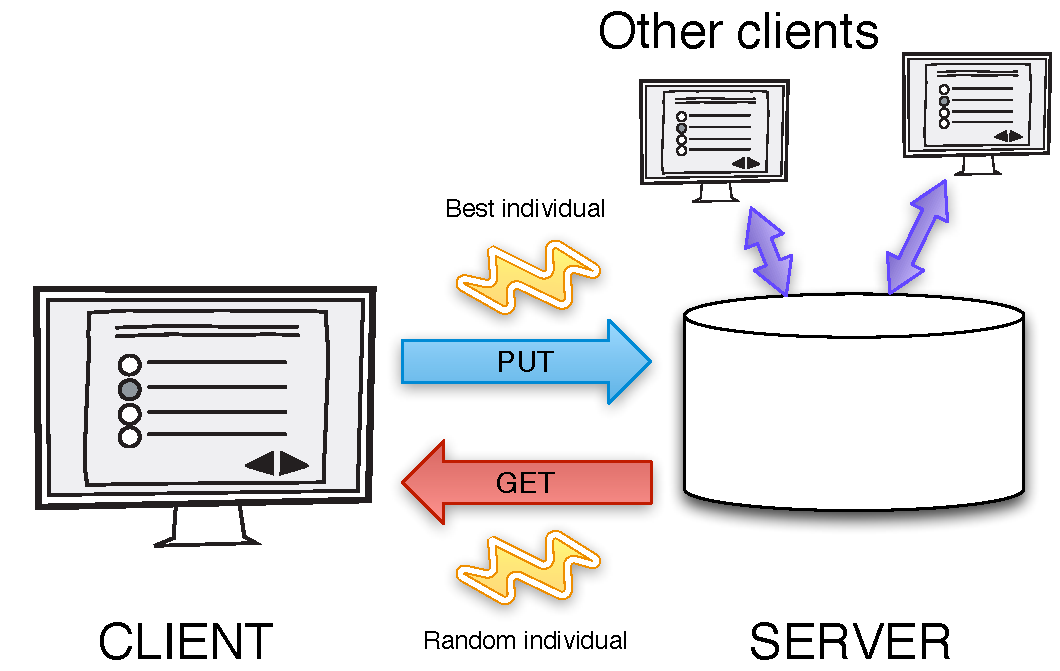
\includegraphics[width=3in]{system.pdf}
\caption{Description of the proposed system. Clients execute a JavaScript EA
  in the browser, which, every 100 generations, sends the best
  individual and receives a random one back from the server.}
\label{fig:system}
\end{figure}

%%%% DELETE? Repeats lines 186 - 191
The researcher only has to change a function, which can be written in
JavaScript or in any other language with cross-compilation to
JavaScript \citep{web:compilersjs} to solve a different
problem. 
%%%%  
In this case the classical Trap function \citep{Ackley1987} has been
used. JavaScript is a functional language and declaring a different 
function and handing at the creation of the algorithm object, called
{\tt Classic}, is the only change needed to work with a different
problem. Let us see how this system addresses the different challenges
outlined in the State of the Art (Section \ref{sec:soa}):
\begin{itemize}
\item {\em Scalability} is provided via the use of a lightweight and
  high-performance, single-threaded, server based in Node.js and
  Express.js. Although this single server is a bottleneck since it
  will eventually saturate, the fact that it runs as a non-blocking single thread
  allows the service of many requests. In fact, a limit in the
  number of simultaneous requests will be reached, but so far it has
  not been found, unlike what we found in our previous systems, DCoR,
  \citep{gecco07:workshop:dcor}, which had a low scalability. 
\item The system is {\em heterogeneous} since it does not need any
  performance, operating system, or even browser requirement as long
  as JavaScript is enabled: anyone
  visiting the page, even from mobile devices, can load the algorithm.
\item {\em Fault tolerance} is always an issue, and in this case, the
  single point of failure would be the server: the system, as such,
  would break down if the server fails. However, the individual
  islands in every browser would continue running, and having access
  to just one of them would allow the local algorithm to proceed. In
  fact, the island does not need the server to run: it runs locally if
  needed, with the only exception that it is obviously unable to
  communicate with the rest of the islands.
\item {\em Adaptiveness} is achieved simply through the autonomous
  operation of every individual island without any synchronization
  mechanism. The islands in the system are, in fact, unaware of each
  other, communicating only through the server. This architecture 
  has been tested in other high demand systems with success, but 
  in the case of {\sf NodIO}, additional experiments are needed to asses 
  the scalability of the communication system. % (Paloma) Is it ok if we talk about scalability when we were talking about adaptiveness? Scalability was also described in the first point.
  %(Mario) Scalability of the communication system in particular?
\item Since the algorithm runs in the browser, {\em safety} is
  achieved through its sandbox mechanisms. The user is thus assured
  that there is no unsafe access either to their local files or even
  to more resources than the browser should be allotted.
\item Running the algorithm is just a matter of loading the page,
  which makes the operation totally {\em anonymous}. For the same
  reason, {\em ease of use} is optimal, being as easy as simply
  clicking on an URL, available to anyone with access to a browser.
\item {\em Reasonable performance} is not ensured. In fact, we should
  make sure that there is a reasonable amount of clients over which
  the performance achieved is better than what you would obtain in
  your own desktop system. If this is not the case, it is a pointless
  academic exercise.
\end{itemize}

There are many different ways to validate a framework that intends to
address these challenges. Some of them are included by design: it is
anonymous, since no accounts are needed to participate in the
experiment, it is safe for the user, since we are using the browser
black box, and it is also heterogeneous. We have designed the
experiments so that they show adaptability to different types of
experiments and clients, scalability with the number of clients and
the problem size, and measured performance by comparing it with
a baseline configuration, with which, as indicated above, is
compatible and can be used in a complementary way. Fault tolerance
will be experimented by dropping the server and checking the continuity
of the experiments. 

All these points will be established in the next two sections,
starting with the baseline, single worker system next. %%%  Single worker? 

%---------------------------------------------------------------
\section{Baseline Experiment and obtained results} %Cambié el nombre
\label{sec:experiments}

\begin{figure}[!t]
\centering
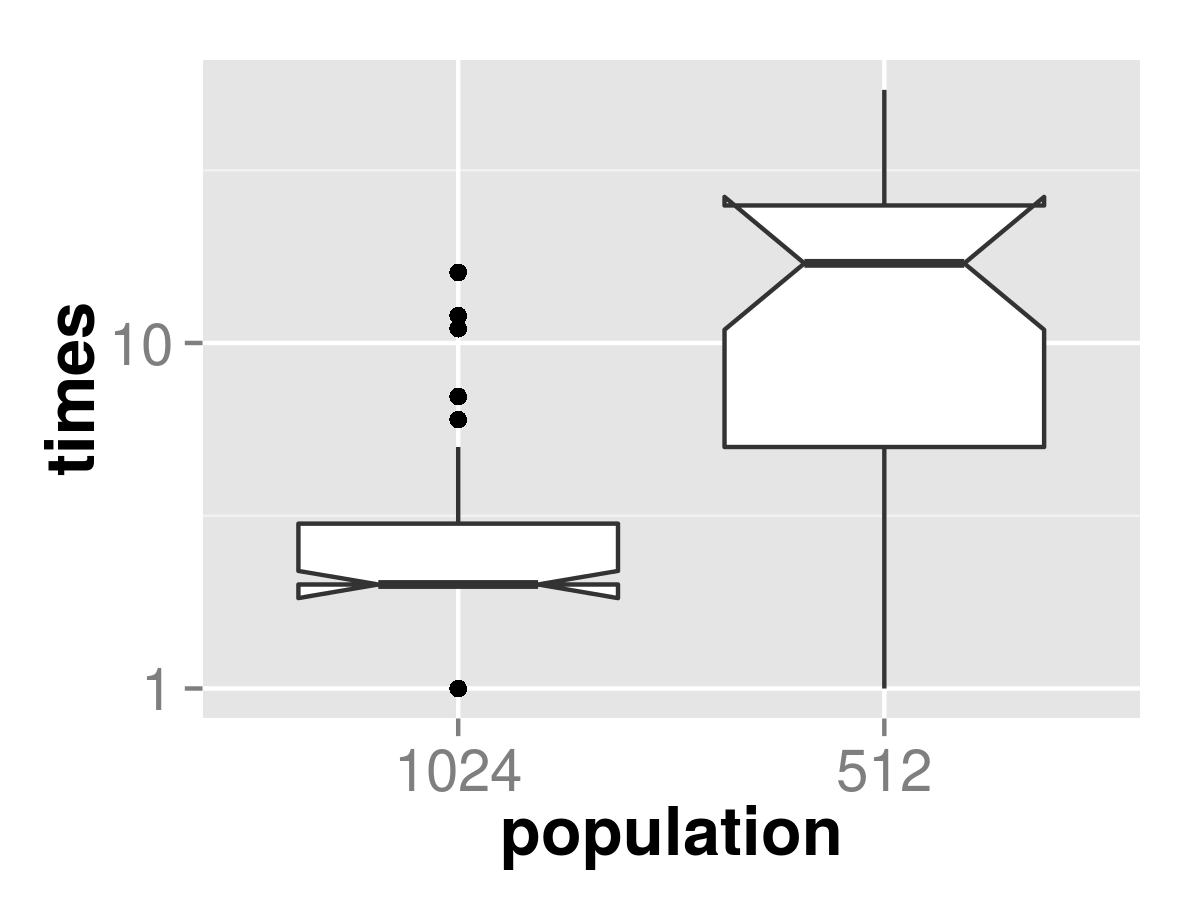
\includegraphics[width=3in]{baseline-times.png}
\caption{Comparison of times to solution (labeled as {\bf times}) for the baseline system, using a {\tt
    Node.js} client, for different population sizes. Only
runs in which solution has been found are used for this graph.}
% Plotted with: ~/Code/splash-volunteer/data/plot-baseline.R
\label{fig:baseline}
\end{figure}
First, we establish the baseline performance by running the
evolutionary algorithm in a desktop client written using {\sf NodEO}
\citep{nodeo2014}, the basic JavaScript library we have used as base to
build {\sf NodIO}, the framework. This experiment tries to 
find the solution to the 40-trap function with parameters $l=4, a=1,
b=2, z=3$ and a population size equal to 512. The algorithm in a
single island was run until the solution (a string with all
ones) was found or five million evaluations had been performed. It
took around a minute, on average, that is $68.9694$ seconds, to
perform the fifty runs. In this experiment only 33, that is, 66\% were
successful. The experiments were repeated for population $p=1024$,
with a success rate upgraded to 100\% and an {\em average} duration of $3.46$
seconds. Results for these two experiments
are shown in Figure \ref{fig:baseline}. The baseline hardware system has these
characteristics: 
\begin{verbatim}
Linux penny 3.13.0-34-generic #60-Ubuntu SMP Wed Aug 13 15:45:27 UTC
2014 x86_64 x86_64 x86_64 GNU/Linux
\end{verbatim}
with a 4-core {\tt Intel(R) Core(TM) i7-4770 CPU @ 3.40GHz}.

These two experiments establish a baseline result and show that
the time to success depends on the population size, with a bigger population
contributing to have more diversity and thus speeding up the solution \citep{DBLP:conf/lion/LaredoDFGB13}. The volunteer computing
experiments that we will describe next do not and can not have the
same conditions, but
the baseline is that if they eventually take longer than a basic
desktop, their interest will be purely academic. We will try and
prove next that that target performance can be achieved by carrying
out several experiments in different conditions. Second, they also act
as a basic performance test for the server, and also prove that the
basic server can be used for many kinds of different setups, as long
as they follow the REST protocol to deposit and obtain individuals
from the pool. It is obvious that, in this case, the server is not
really needed, since there is a single client and no interaction
between them, but there is a cost in sending and obtaining chromosomes
from the server so it is included for the sake of fairer comparison.

\subsection{Volunteer evolutionary computation: first experiments and results}

Initial experiments were set up using the OpenShift
PaaS, which provides a free tier within which this 
experiment could be performed. That way, and as required, the hardware
and cloud cost for this experiment were zero. Experiments were
announced through a post in Twitter and other social networks, and
results were published here \citep{DBLP:conf/gecco/GuervosG15}. For the
purpose of this paper, we repeated the announcement several times
through the month of April and then by the beginning of August. All
in all, we have the set of runs with the characteristics shown in
Table \ref{tab:runs}. In general, every experiment took several
days. No particular care was taken about the time of the announcement
or the particular wording. Every {\em experiment} consisted in running
until the solution of the 40-trap problem was found. When the correct
solution was sent to the server, the counter was updated and the pool
of solutions reset to the void set. There was no special intention to wait
until all clients had finished, thus it might happen that, in fact,
the islands running in the browser {\em spill} from one experiment to
the next. However, previous experiments have proven that the influence
of these islands in the next experiment is indeed negligible.
%
\begin{table*}
\caption{Characteristics of the volunteer computing initial runs. \label{tab:runs}}
\begin{center}
\begin{tabular}{l|rr}
\hline
Date & \# experiments & Different IPs \\
\hline
April 4th 4/4 & 57 & 191 \\
April 24th 4/24 &  231 & 559 \\
July 31th 7/31 & 97 & 179 \\
\hline
\end{tabular}
\end{center}
\end{table*}
%
\begin{table*}
\caption{Summary of time per run, number of IPs and number of {\tt
    PUT}s per IP in the initial runs. \label{tab:summary:os}}
\begin{center}
\begin{tabular}{l|ccccccc}
\hline
Date & Median \#IPs & Max \#IPs & Median time (s) & Median \#{\tt
  PUT}s & $<$ 69s & $<$ 3.46s & Inter-exper. correlation\\
\hline
4/4 & 5 & 16 & 2040 & 18 & 14.29\% & 5.36\% & 0.0082 \\
4/24 &  5 & 29 & 732 & 11 & 47.39\% & 3.91\% & 0.0934\\
7/31 & 5 & 14 & 260 & 23 & 27.08\% & 1.04\%  & 0.1741\\
\hline
\end{tabular}
\end{center}
\end{table*}
%
The table shows that every run included more than 50 experiments. The
number of different IPs intervening in them varied from more than one
hundred to more than five hundred in the second experiment.

A summary of the results of each run is also shown in Table
\ref{tab:summary:os}, which shows the median number of IPs
intervening in each experiment,  median time needed
to finish the experiment, median number of HTTP {\tt PUT}s per IP, and
then two columns showing the percentage of experiments that took less
than the two baseline experiments shown in the introduction to this
section. The first striking result is that in all cases, 50\% of the
experiments involved 5 or less IPs. This is consistent with results
previously obtained \citep{DBLP:conf/gecco/GuervosG15} which found 6 to be
the usual number of IPs that participated in an experiment. The
maximum number of different IPs for each experiment is also in the
same range and of the order of 10, which is also consistent with
prior work. The median time has a big range of variation, but 50\% of
the time takes less than several minutes, from around 4 minutes in the
best case to roughly 2/3 of an hour in the worst case. That figure is
not competitive, {\em a priori}, with the baseline experiment, that is
why it is interesting to look at the columns which measure
the percentage of experiments in which the solution was found in less
time than the baseline. It is similar in all three cases, with around
20\% on average for the first baseline experiment, roughly 3\% in the
second case. The comparison is not totally fair: this experiment takes
place in a browser, and in fact most of the time is devoted to
presenting the charts; the server is also not the same since it is run in a
PaaS instead of a high-performance desktop computer, and it is also a
remote server, not a local server as in the baseline experiment. But
even in this case, we were looking for creating a framework that
allowed us to run evolutionary computation experiments {\em faster} than
in our very own computer. And the results indicate that although it will
happen in 1 out of roughly 5 or roughly 20 cases, depending on what baseline
experiment you choose, it will not happen always or even most of
the time. One of the problems is shown in the last column, which
indicates the statistical correlation between the number of IPs
participating in one experiment and the next. In all cases,
correlation is so low as to affirm that there is almost no
relationship between them, that is, computing nodes are not {\em
  staying} after the solution has been found. This is a feature of
this implementation: the user has to actively reload the page to make
the evolutionary algorithm start again. Thus, the user can decide if to 
continue sharing resources or not. % (Paloma) Feature or disadvantage?
However, it puts a probably            % (Mario) Feature if you only want to share your CPU a little  
unnecessary upper limit on the time, or number of experiments, that a user
will voluntarily perform.

\begin{figure}[!htb]
\centering
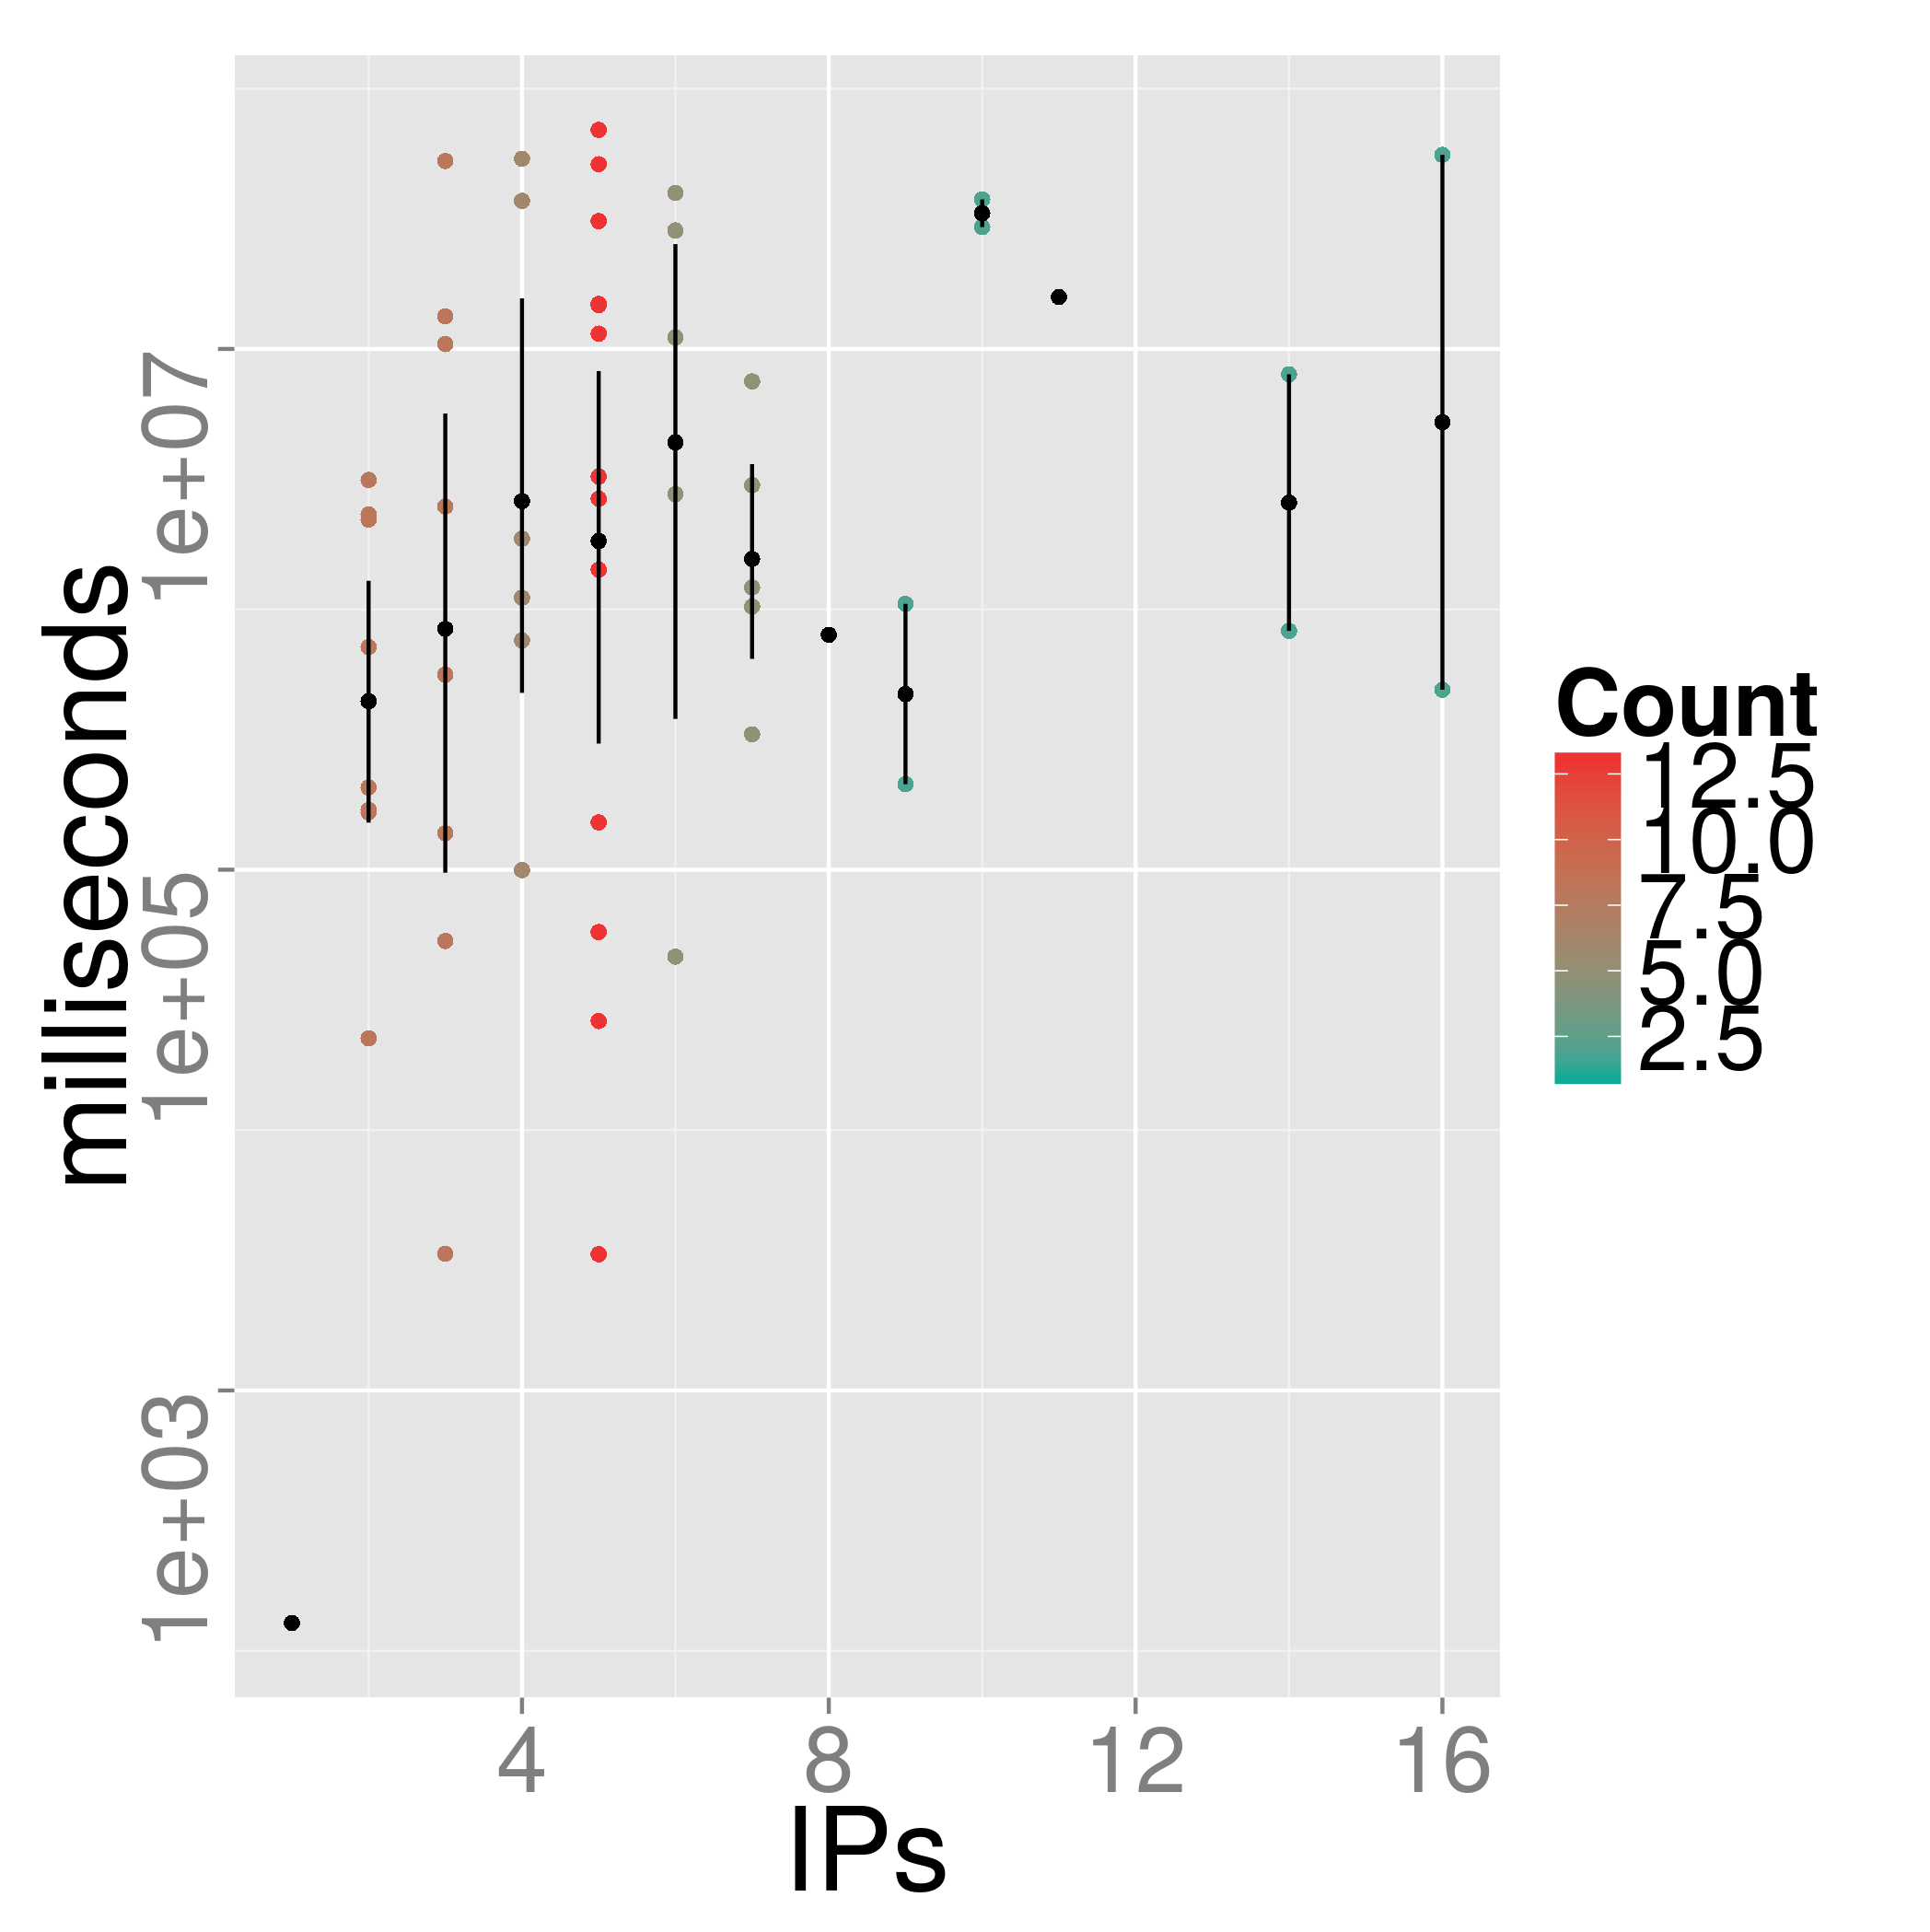
\includegraphics[width=0.32\linewidth]{time-vs-ips-OS-4-4.png}
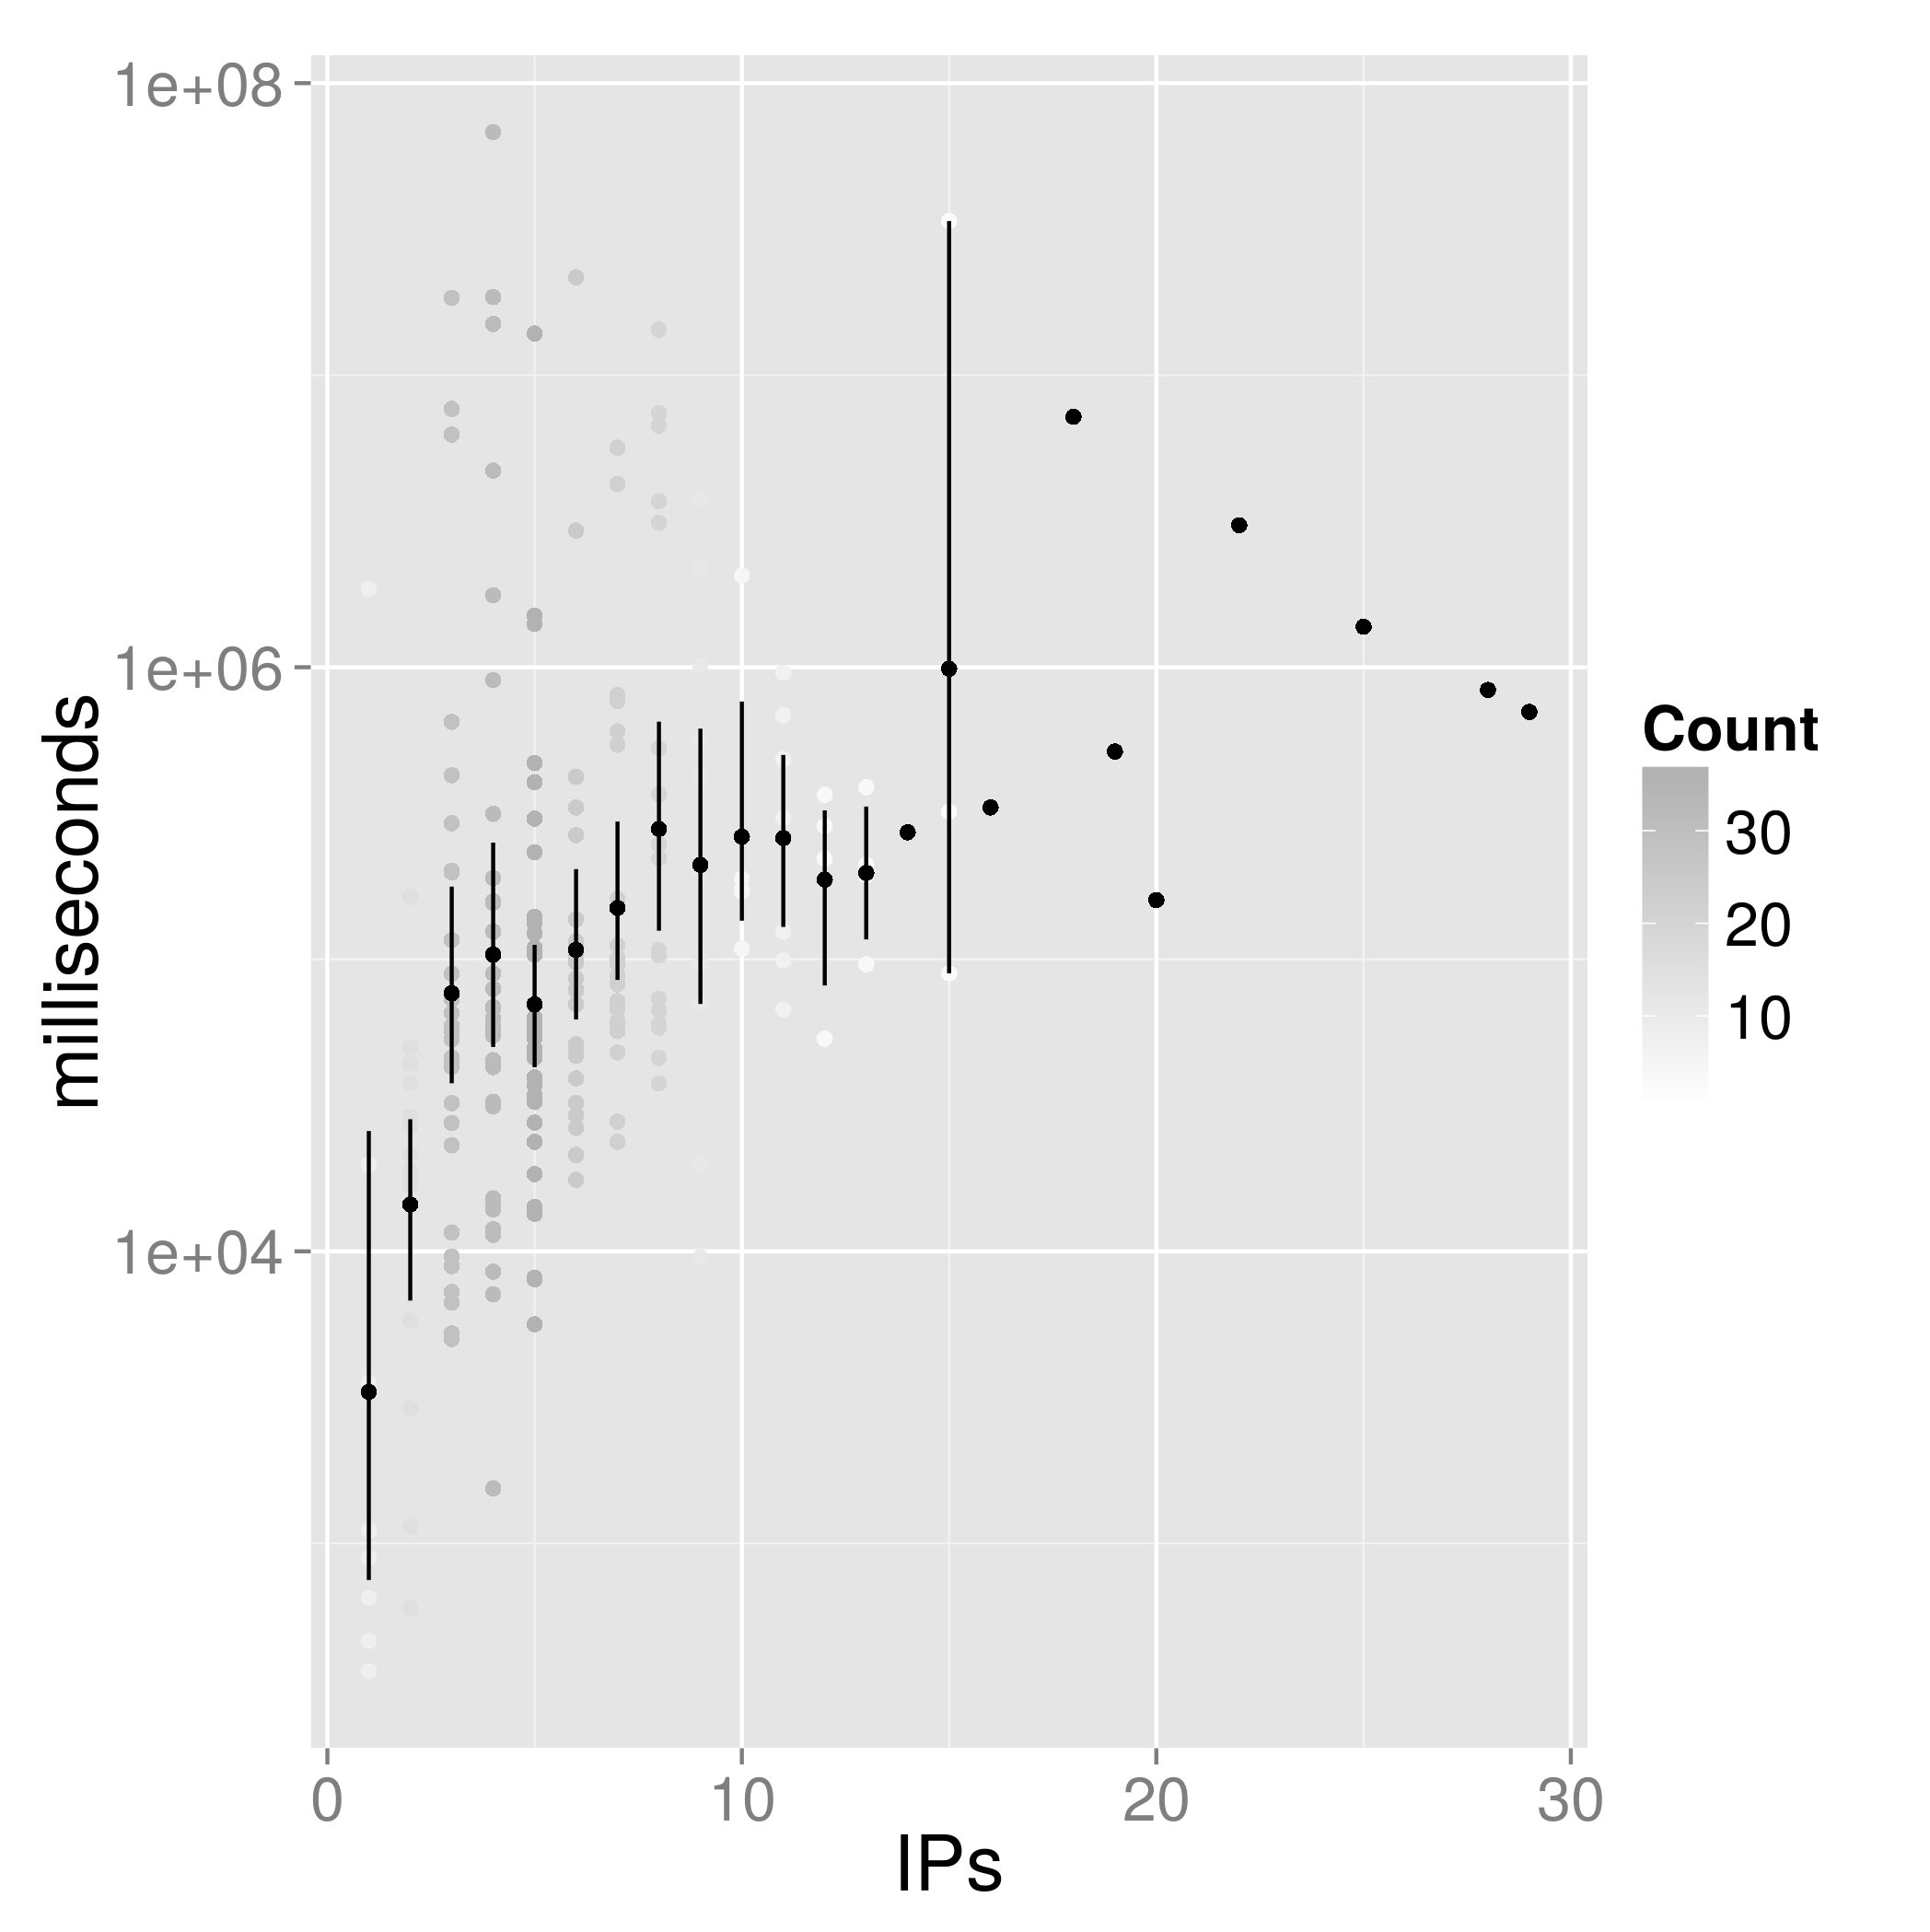
\includegraphics[width=0.32\linewidth]{time-vs-ips-OS-4-24.png}
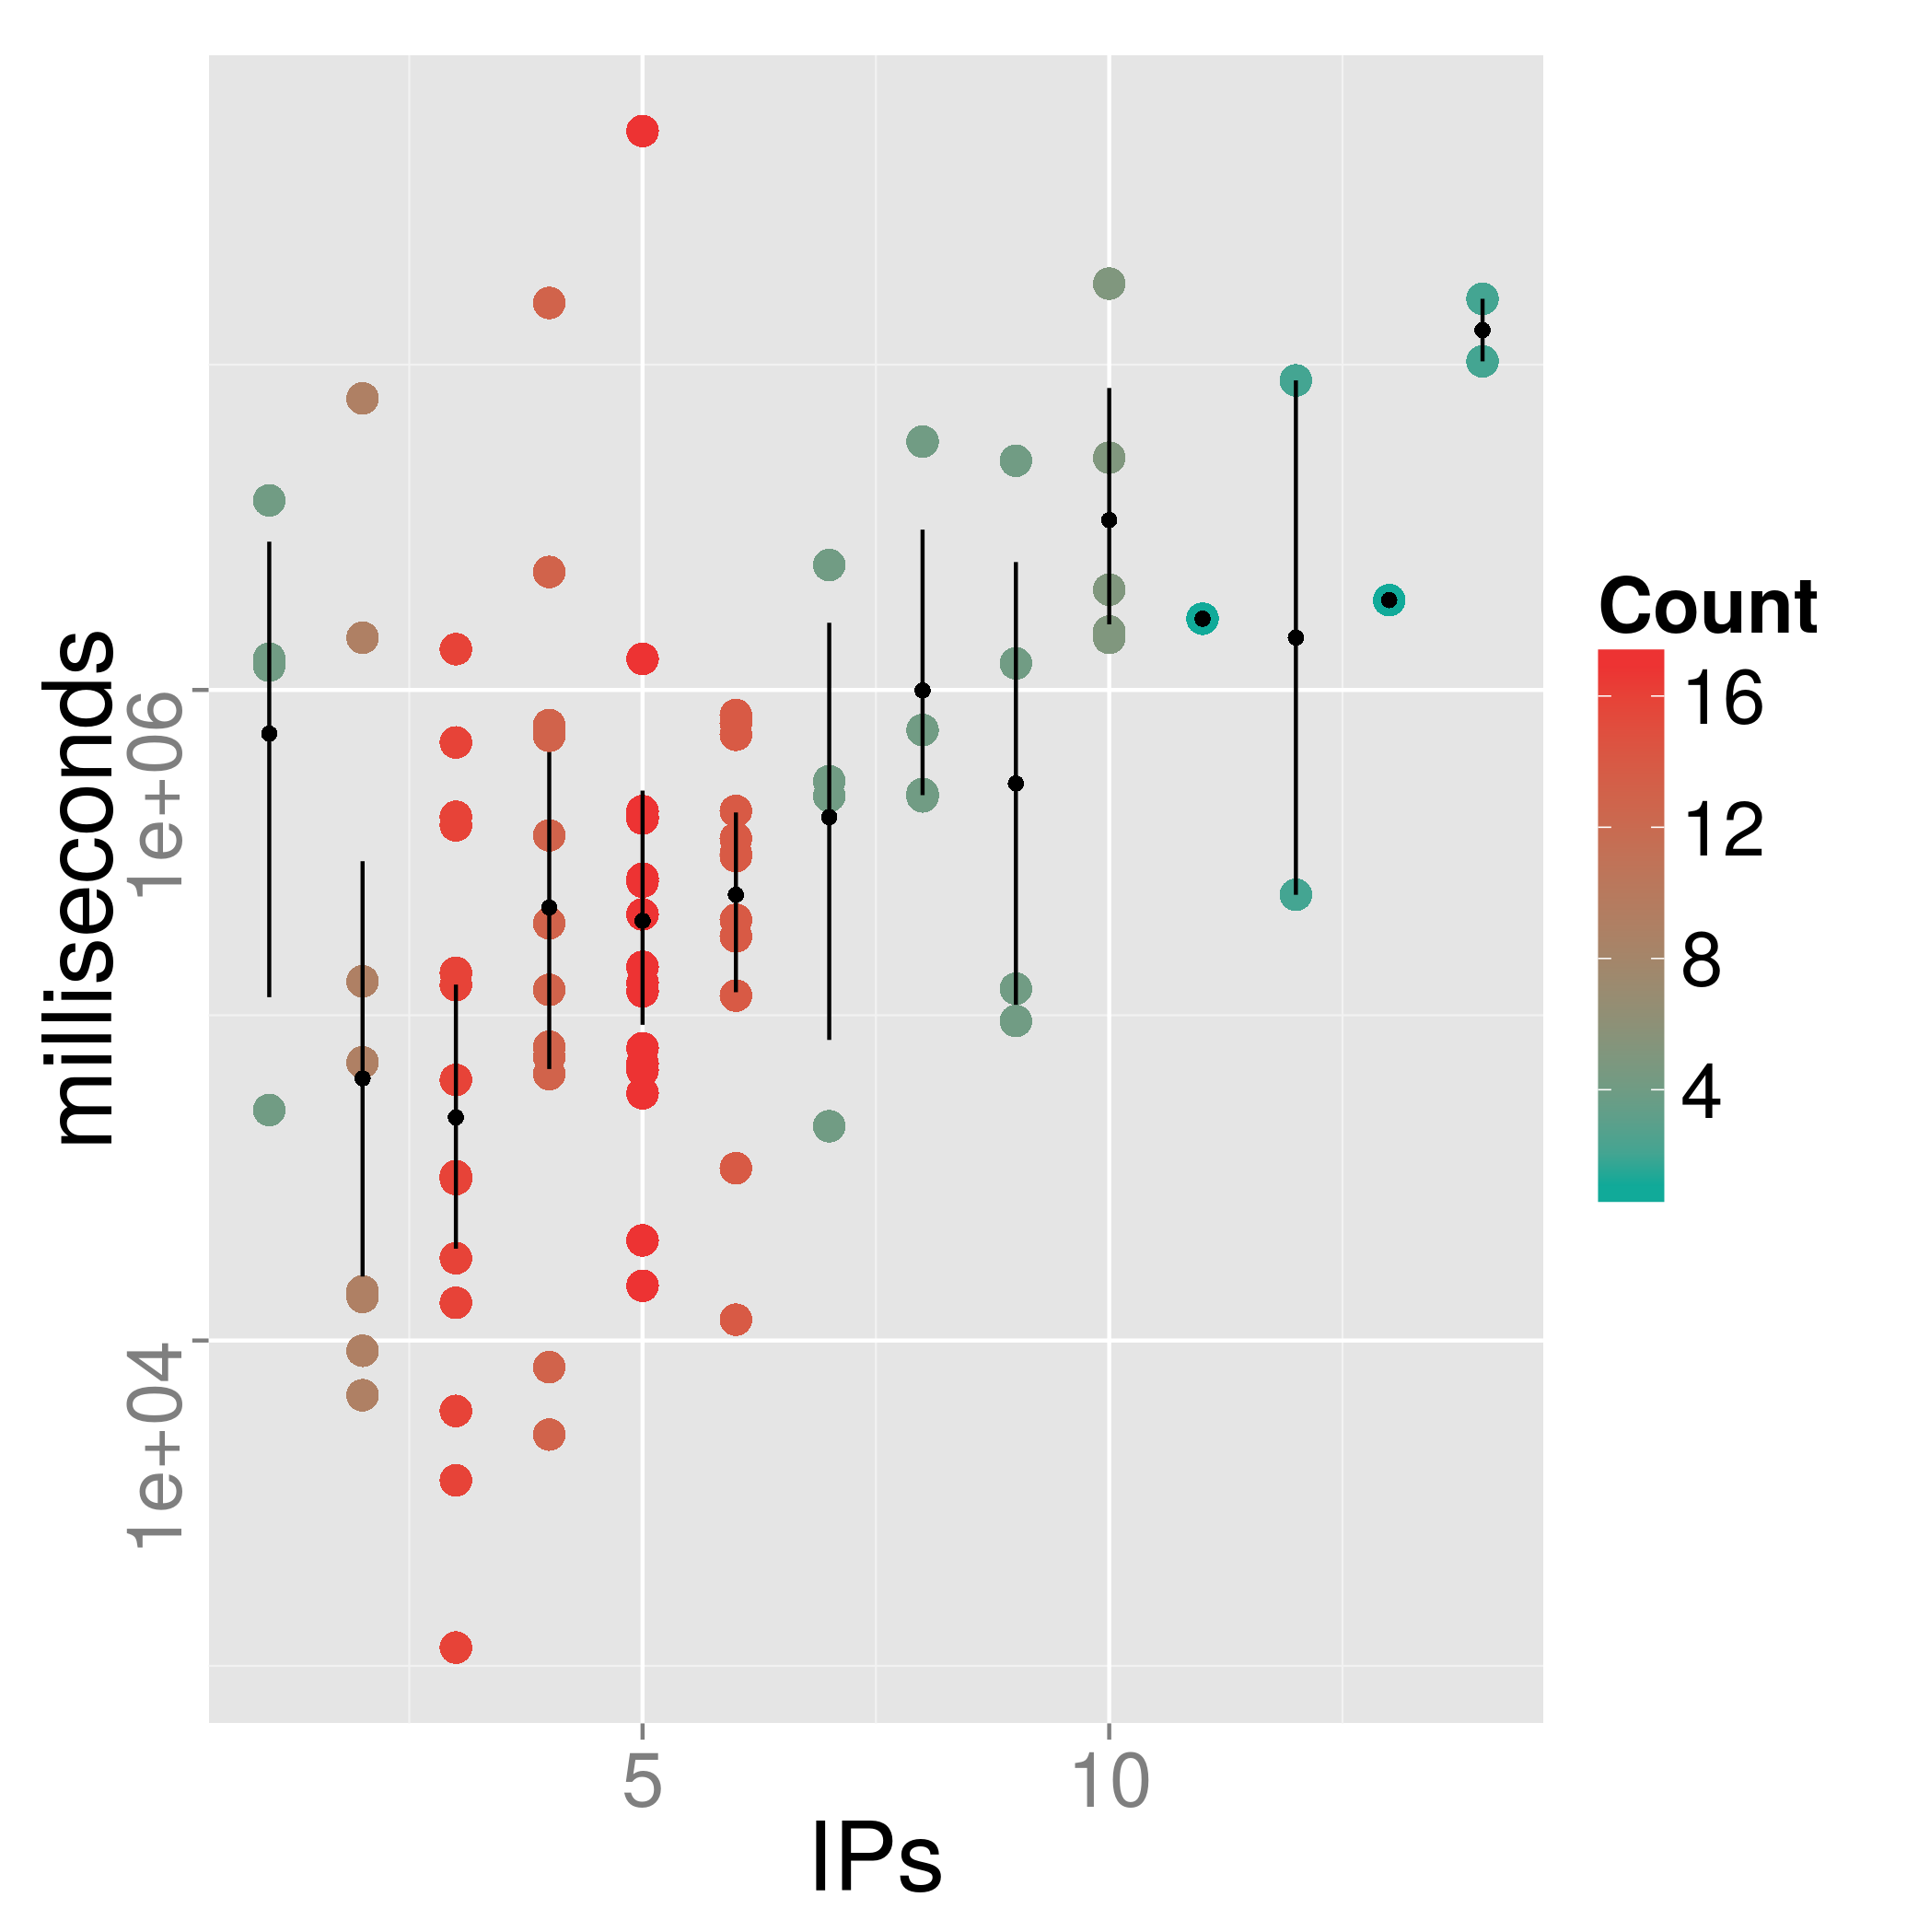
\includegraphics[width=0.32\linewidth]{time-vs-ips-OS-7-31.png}
\caption{Duration of experiments vs. number of different IPs (nodes)
  participating in it, with averages and standard deviation shown as
  red dots; in the case there is a single red dot, there was a single
  experiment in which many computers participated (for instance, 16
  computers in the experiment in the far left or 29 in the middle
  one). 
Shades of blue indicate how many experiments included that many unique IPs,
so lighter shade for a column of dots indicates that a particular number
of computers happened less frequently, while darker shadow means more frequency. 
From left to right, experiments 4/4, 4/24 and 7/31.}
\label{fig:duration}
\end{figure}
%
\begin{figure}[!htb]
\centering
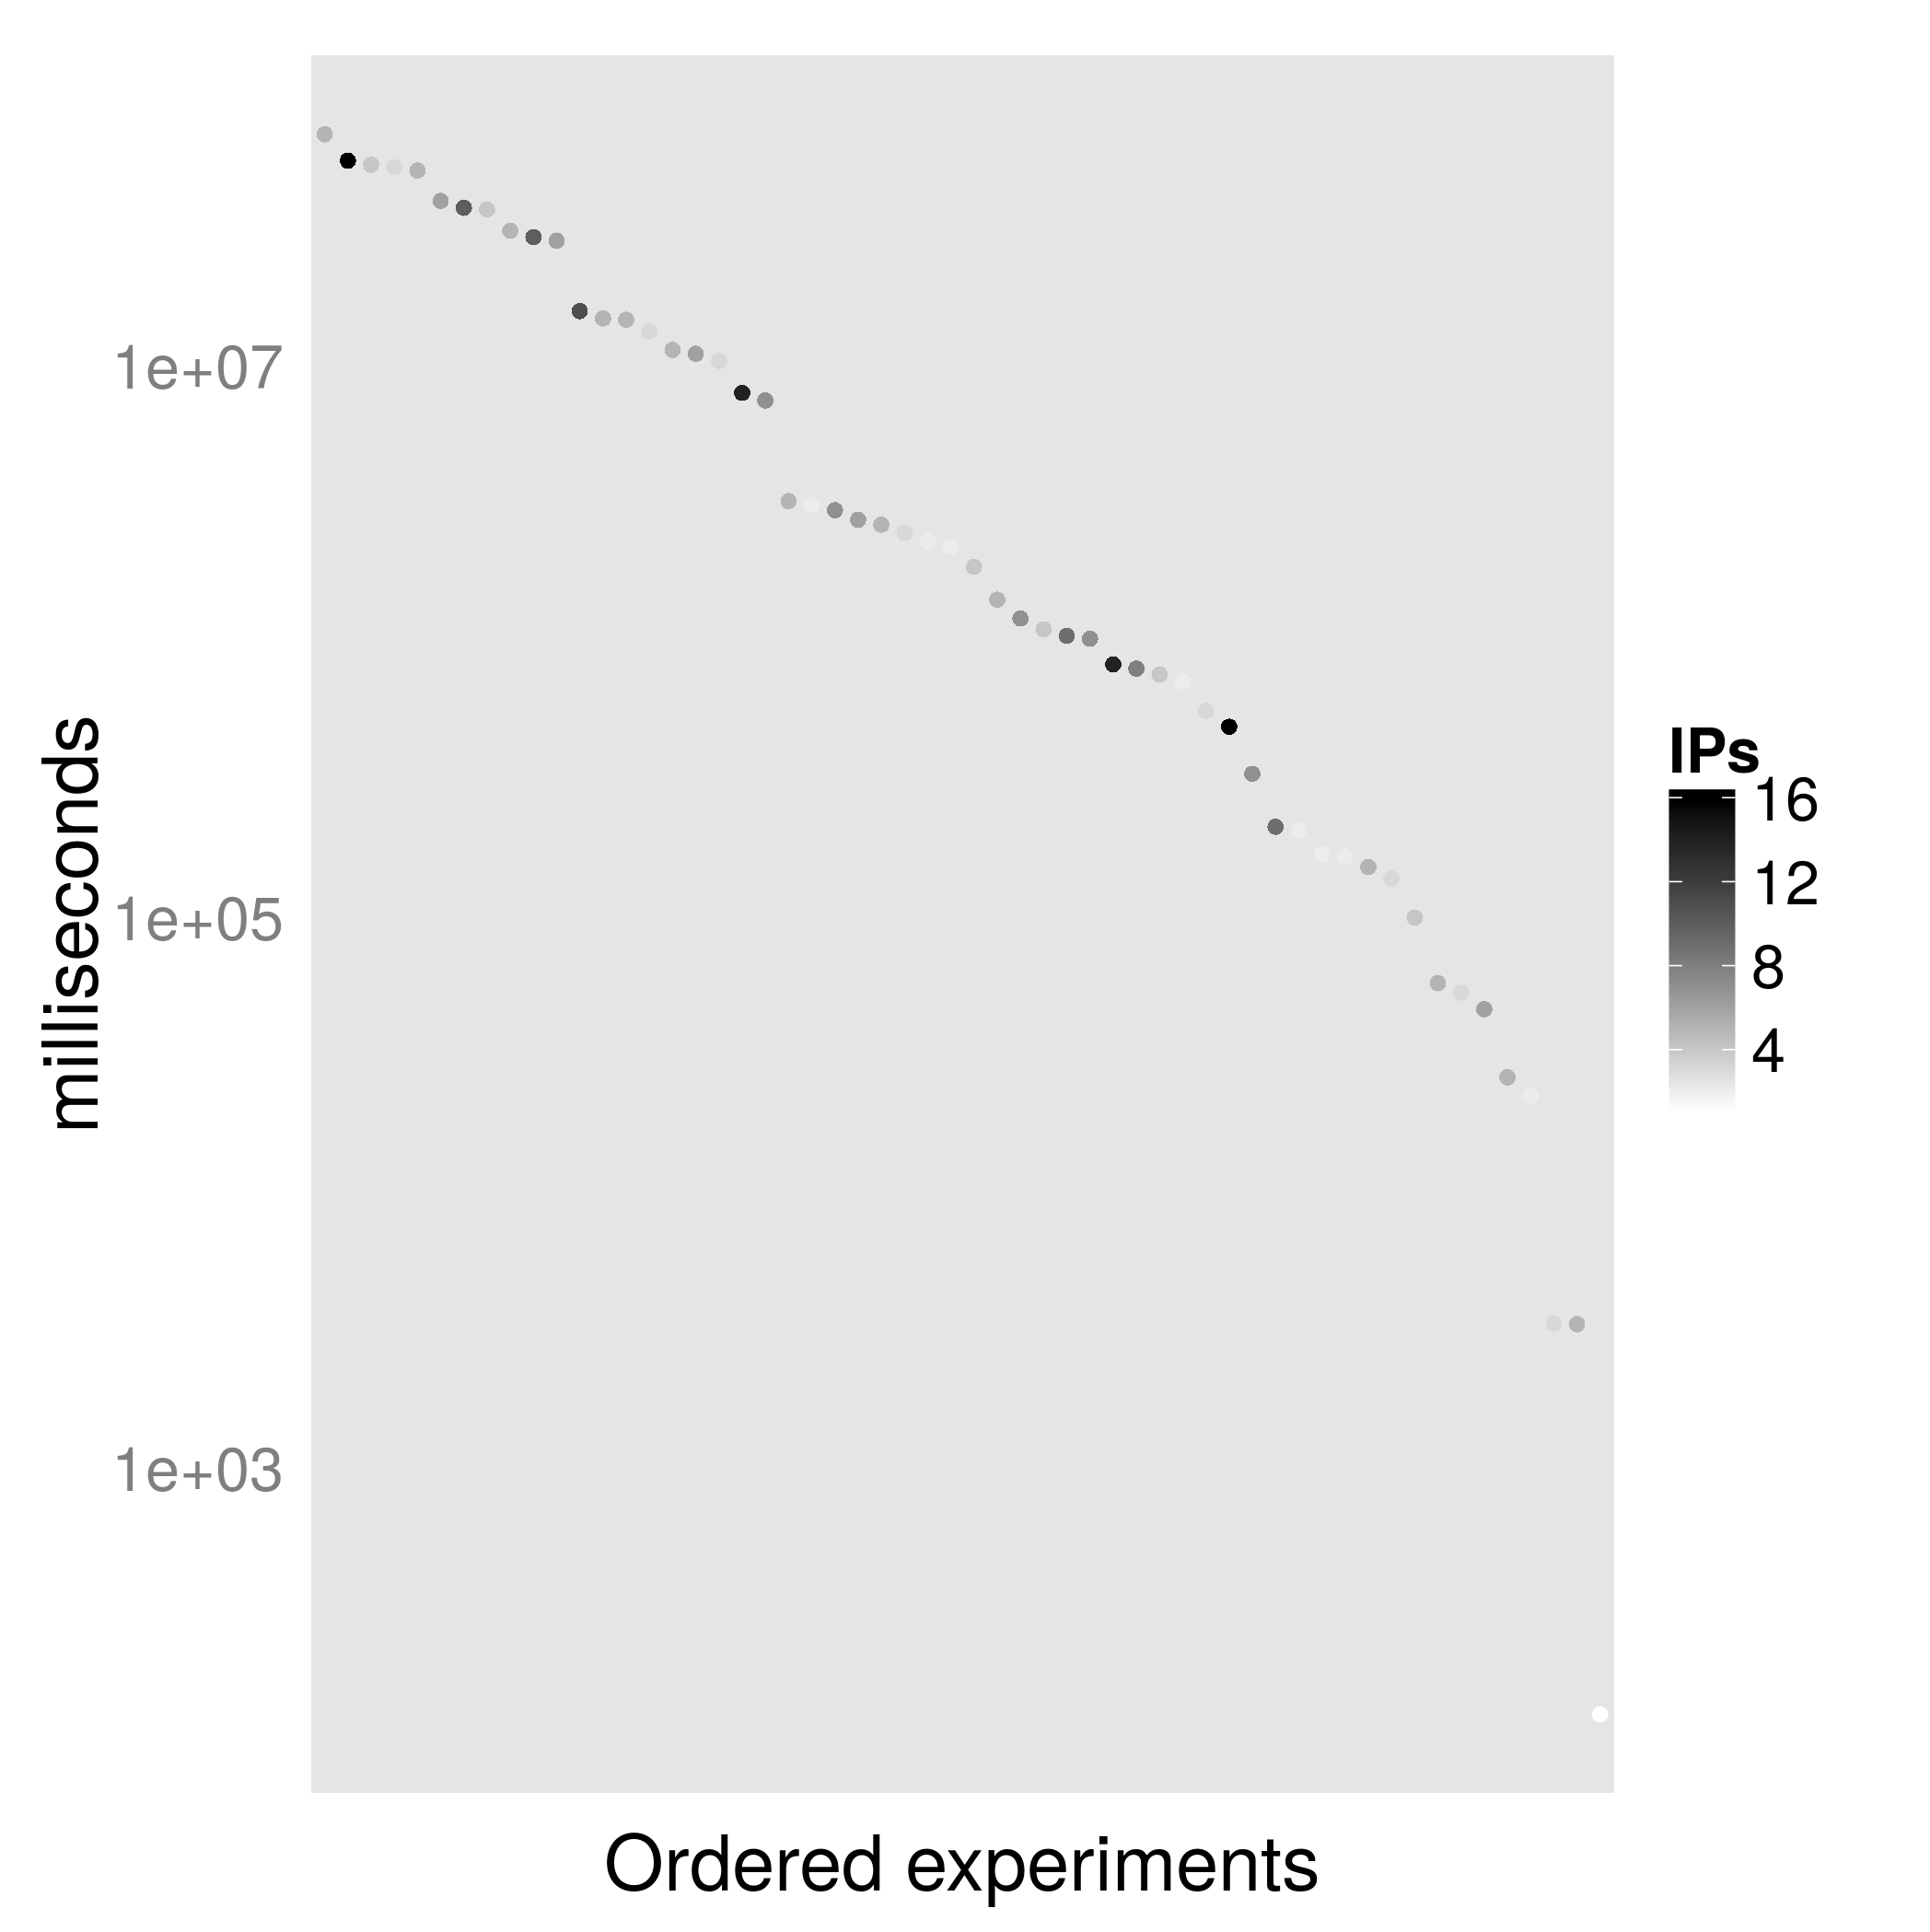
\includegraphics[width=0.32\linewidth]{time-vs-rank-OS-4-4.png}
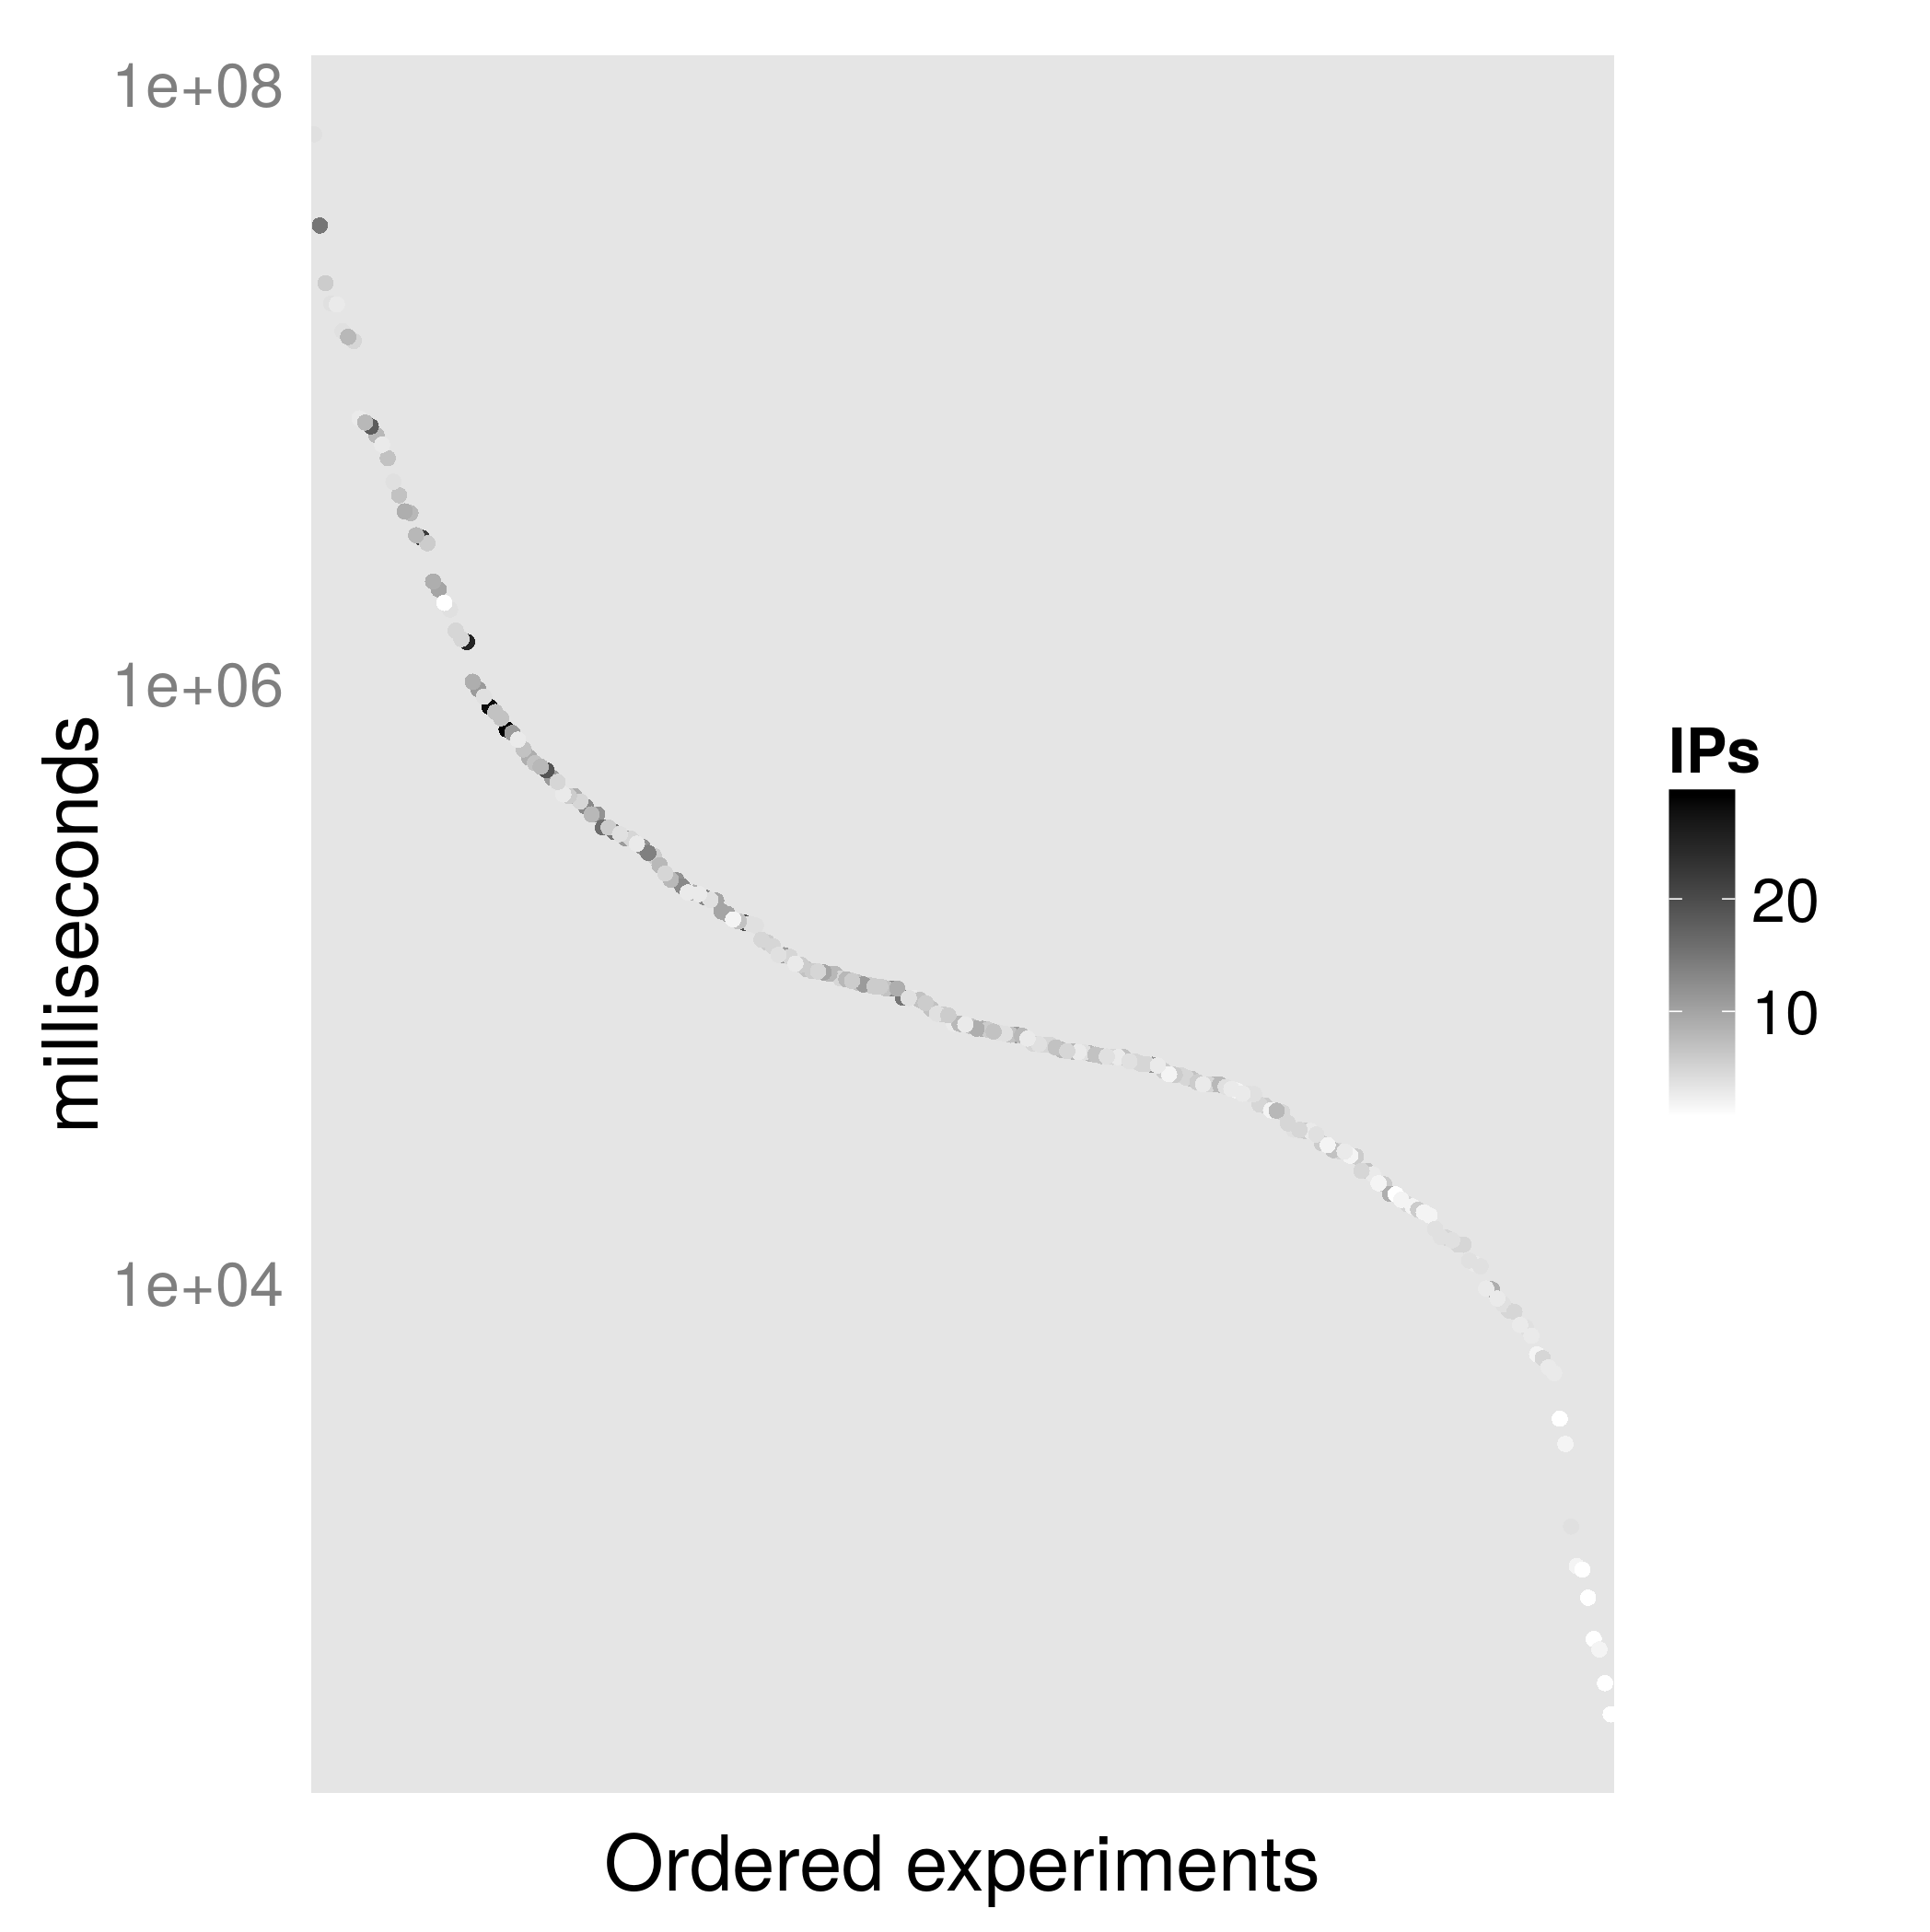
\includegraphics[width=0.32\linewidth]{time-vs-rank-OS-4-24.png}
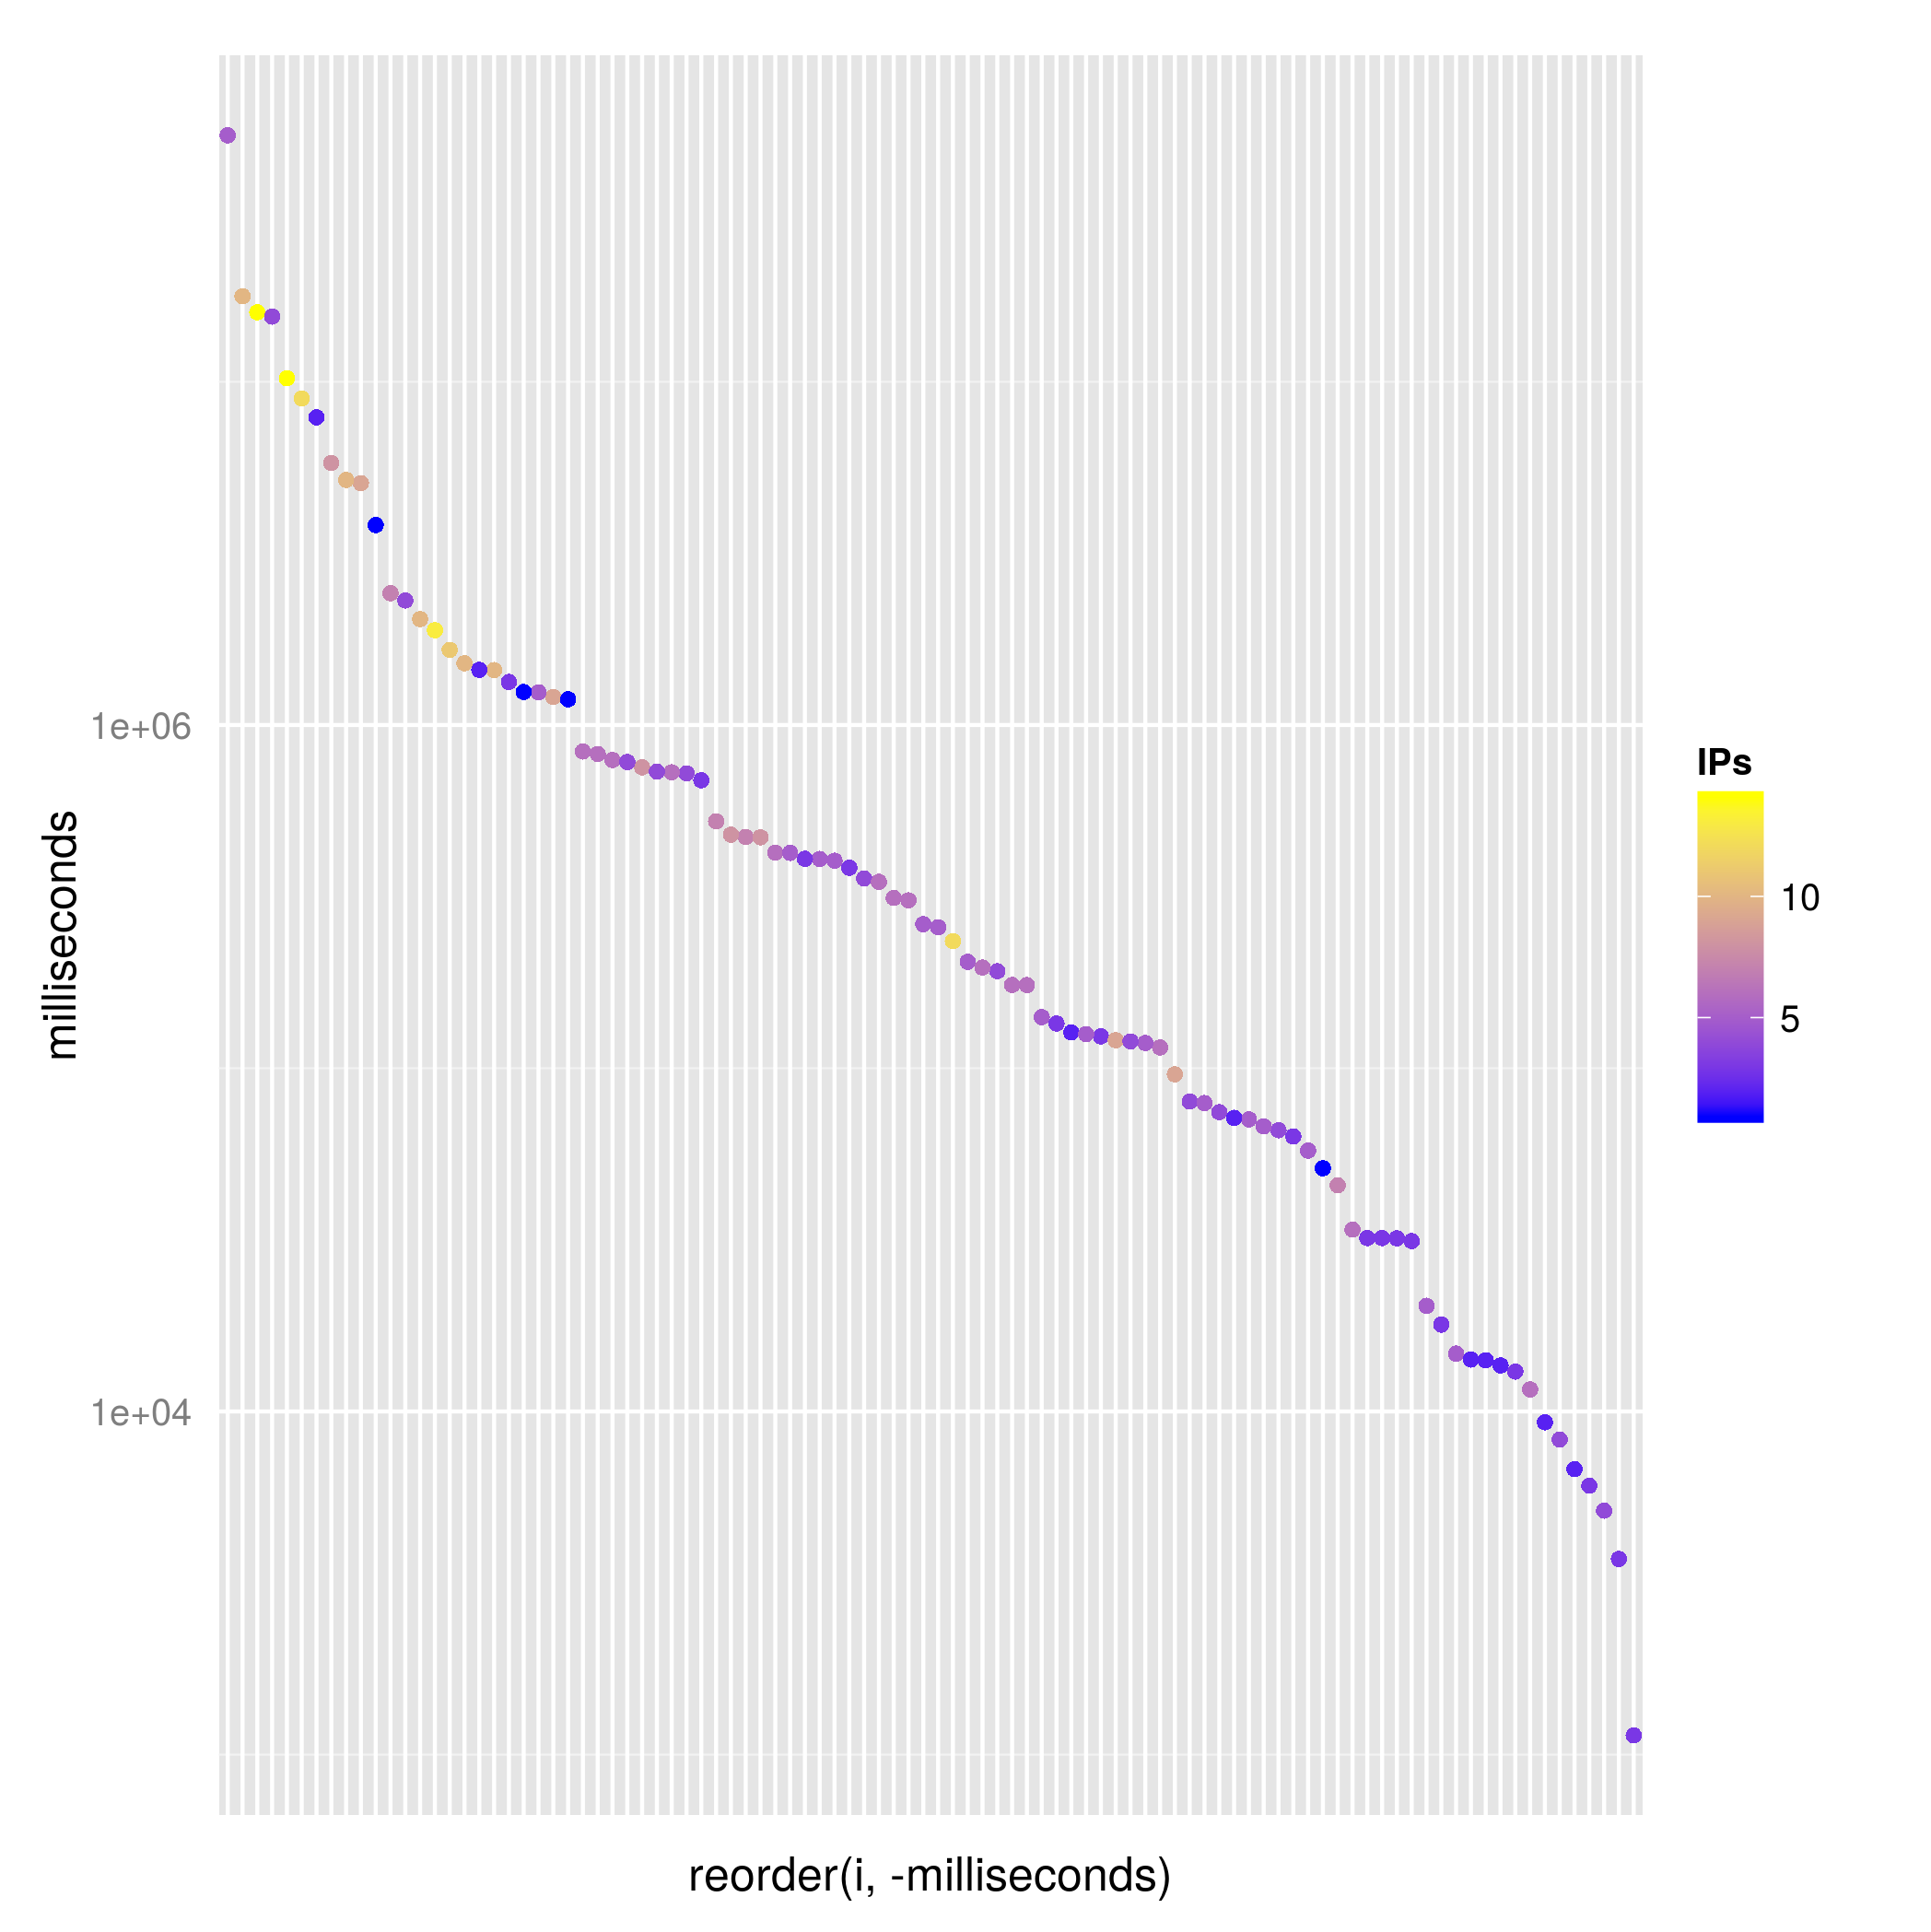
\includegraphics[width=0.32\linewidth]{time-vs-rank-OS-7-31.png}
\caption{Duration of experiments vs. rank, with $y$ axis in a
  logarithmic scale. Dot color is related to the number of IPs
  participating in the experiment. From left to right, experiments
  4/4, 4/24 and 7/31.} 
\label{fig:zipf:os}
\end{figure}
%
We will have to analyze experimental data a bit further to find out why
this happens and also if there are some patterns in the three sets of
experiments. An interesting question to ask, for instance, is if
by adding more computers makes the experiment take less. In fact, as
shown in Figure \ref{fig:duration}, the {\em addition} of more computers does
not seem to contribute to decreasing the time needed to finish the
experiment. However, the cause-effect relationship is not clear at
all. It might be the opposite: since experiments take longer to finish
and might in fact be abandoned with no one contributing for some time,
that increases the probability of someone new joining them. In fact,
with experiments taking a few seconds and due to the way the
experiments are announced, it is quite difficult that several
volunteers join in in such a short period of time, even more if we take
into account that volunteers are not {\em carried over} from previous
experiments. This implies that it would be convenient to use a problem
of a bigger size to check this hypothesis as we have done in the next
experiment. 
%  however, at this point we
% have not found this convenient since there are several other issues
% that have to be solved, as it will be shown next. %Creo que este párrafo
%saldría sobrando ahora que hicmios un experimento más grande

\begin{figure}[!htb]
\centering
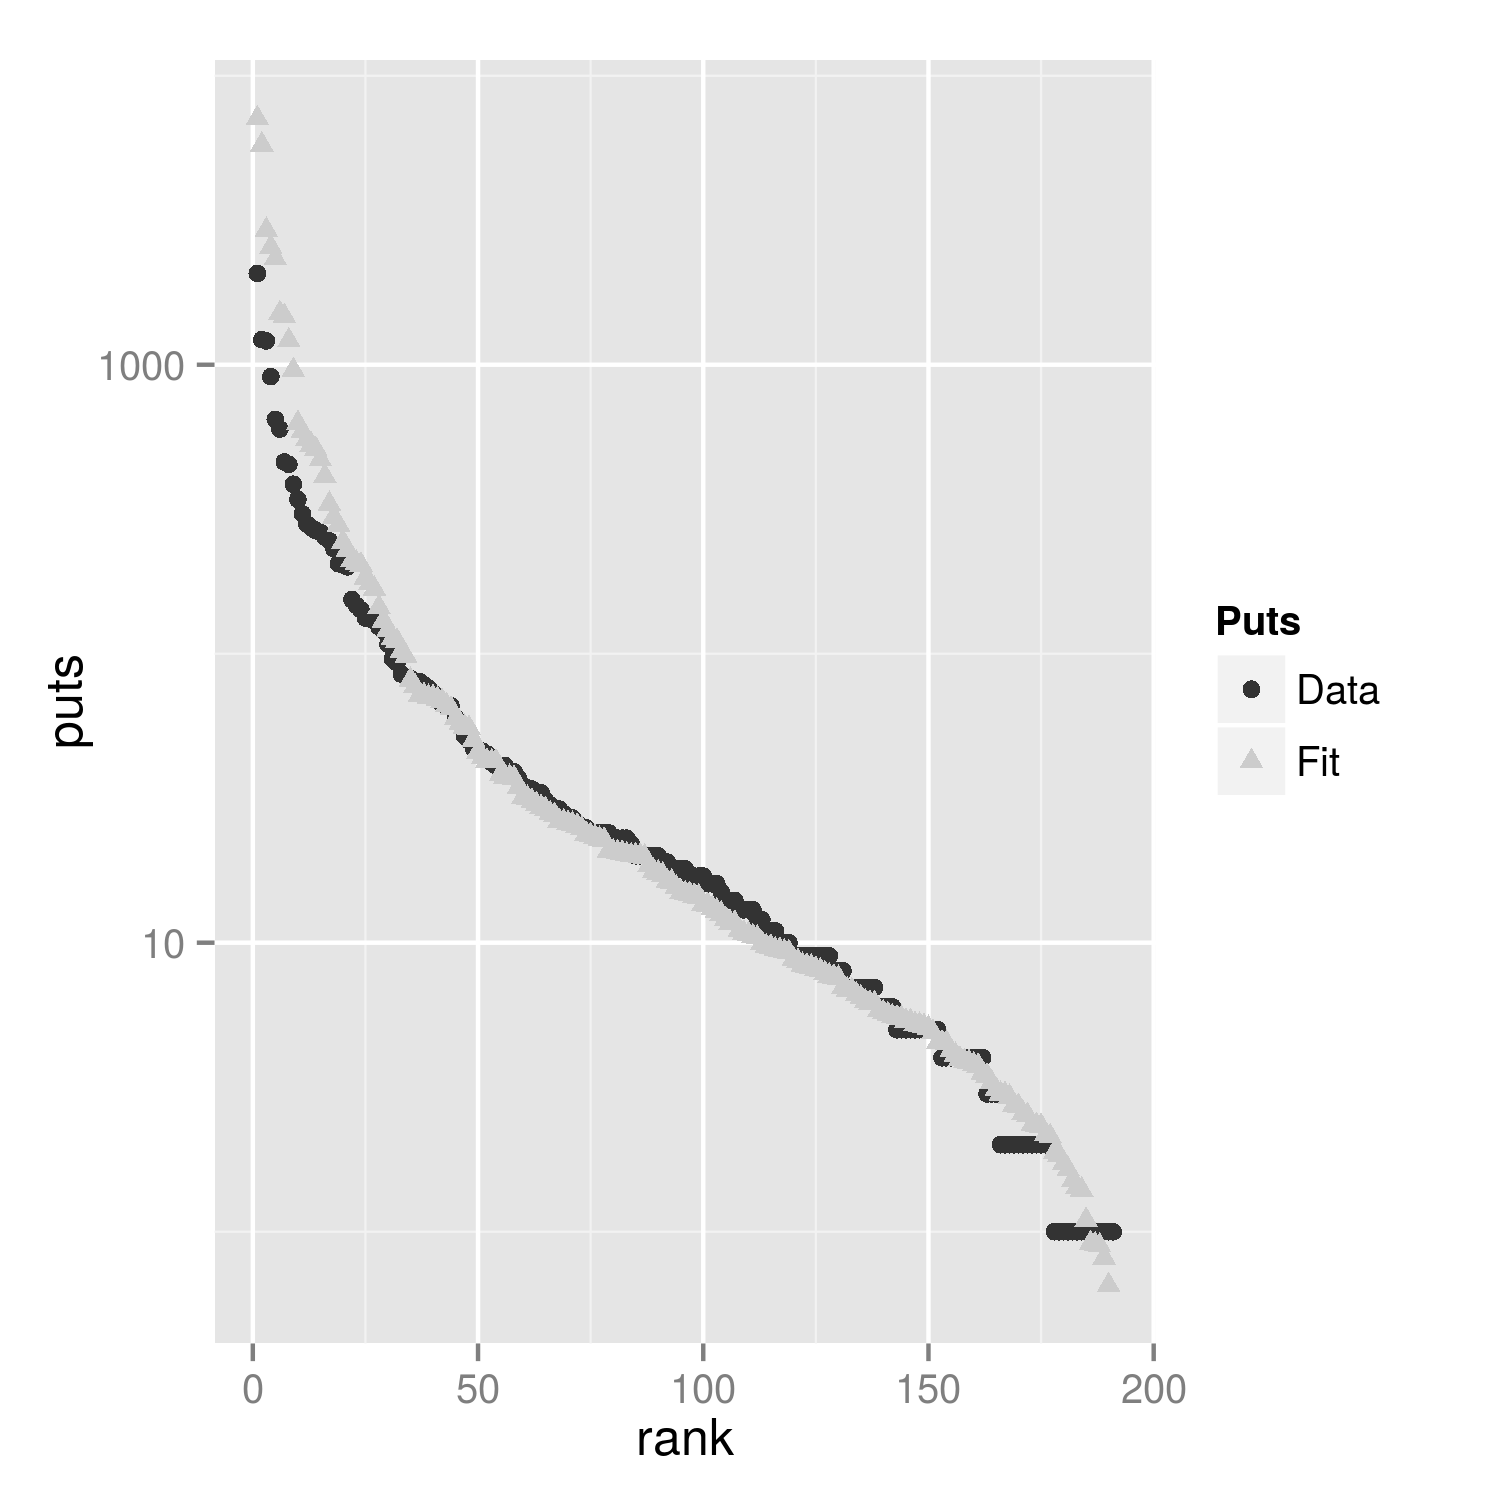
\includegraphics[width=0.32\linewidth]{puts-openshift-4-4.png}
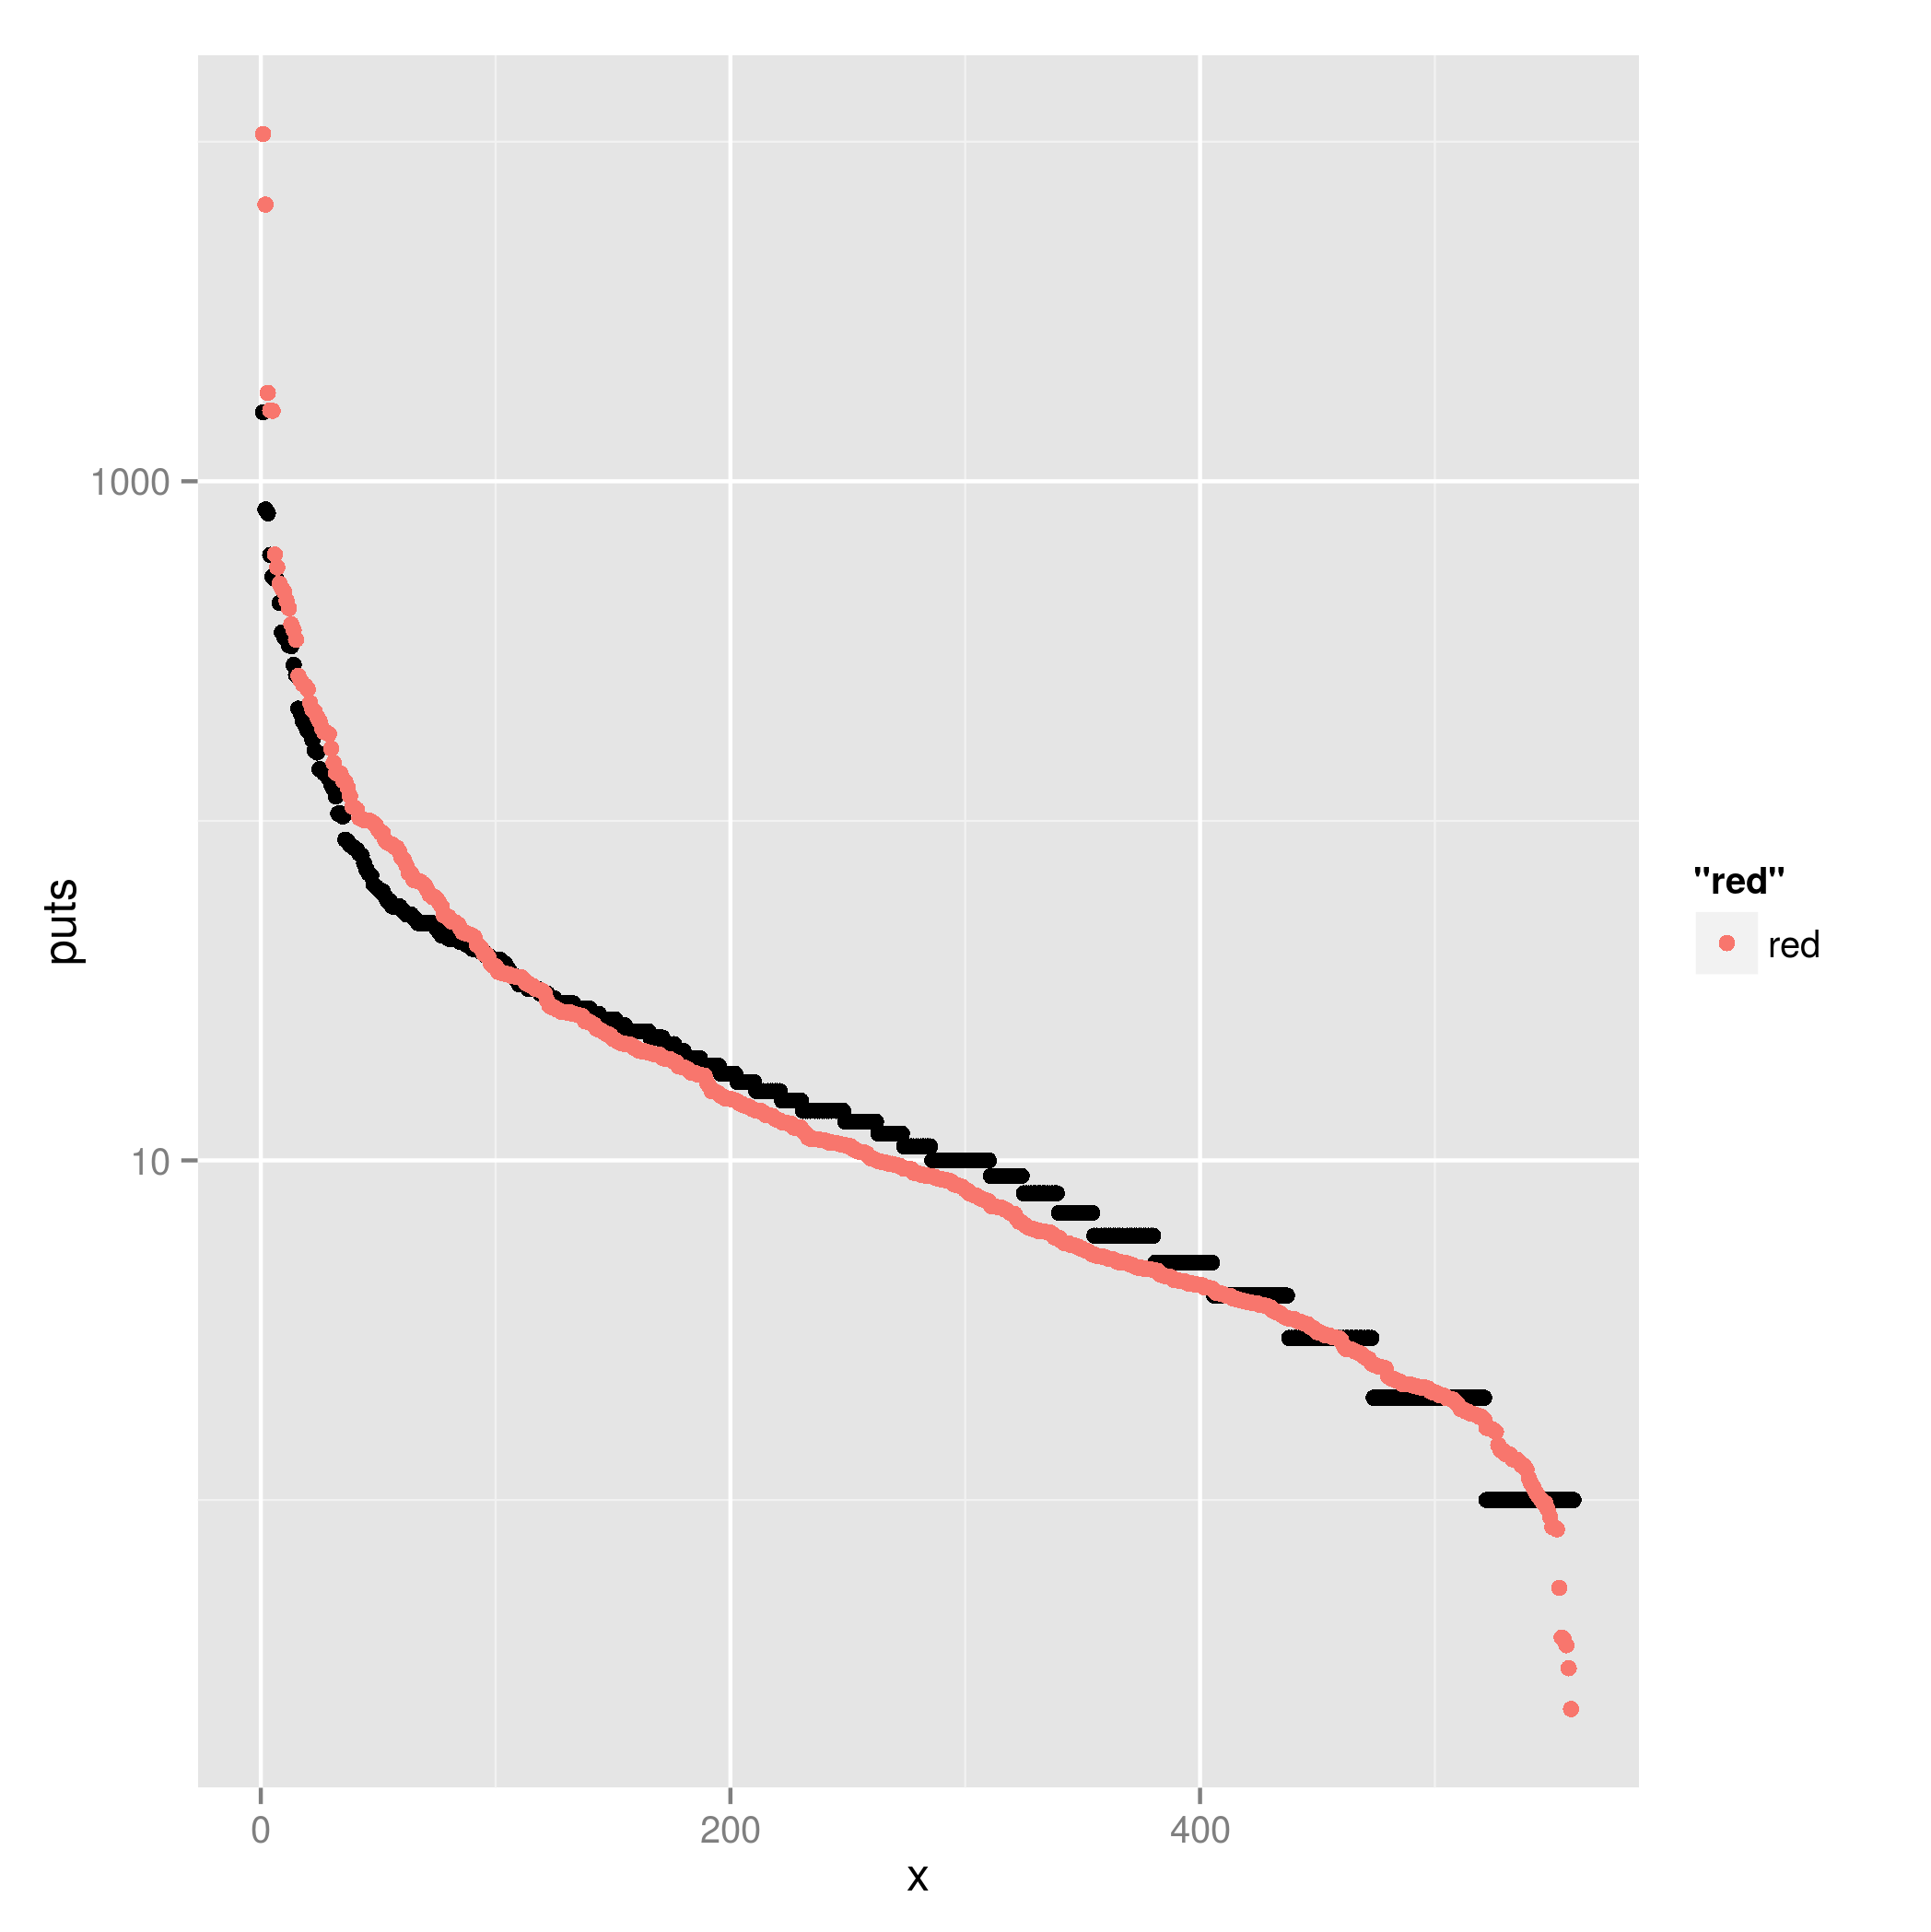
\includegraphics[width=0.32\linewidth]{puts-openshift-4-24.png}
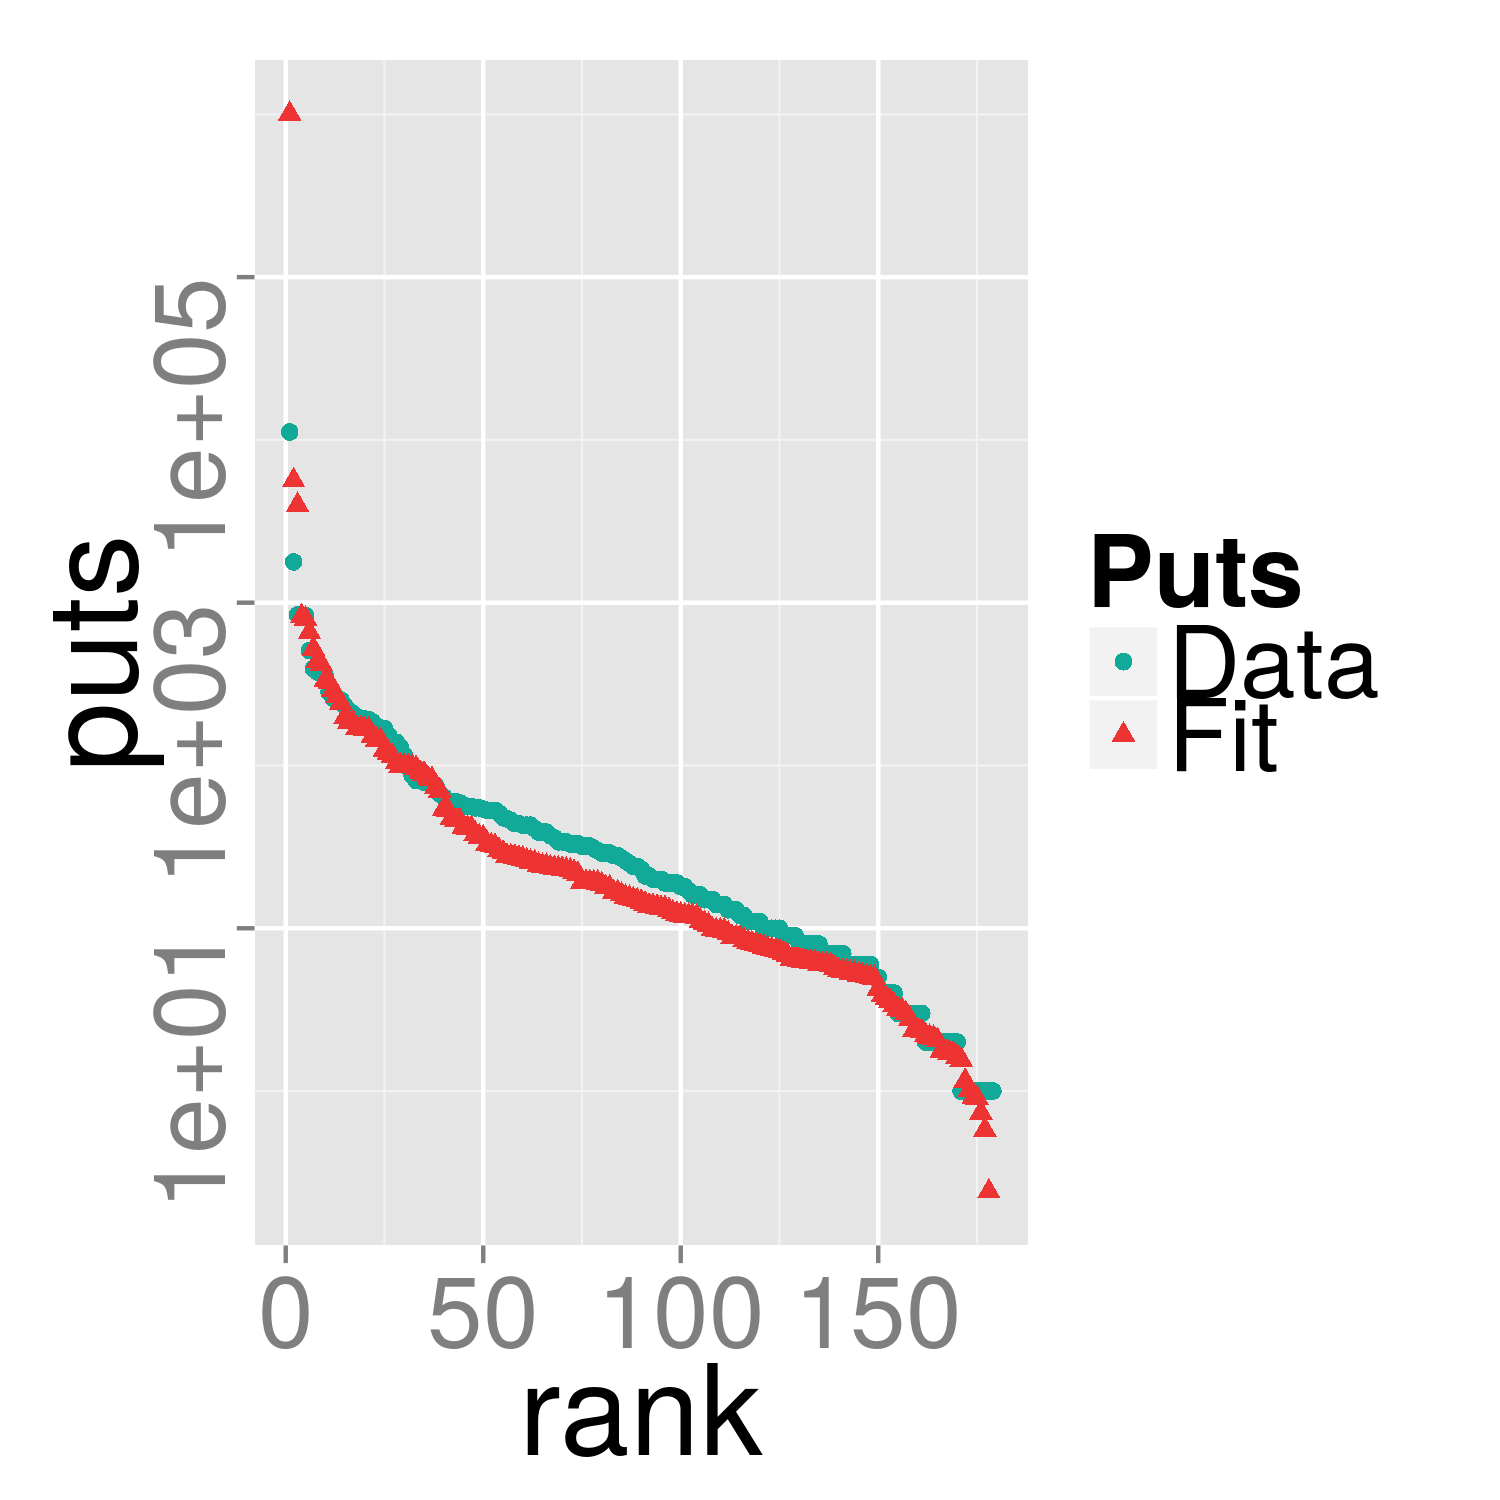
\includegraphics[width=0.32\linewidth]{puts-openshift-7-31.png}
\caption{Number of {\tt PUT}s per unique IP and fit to a Generalized
  Extreme Value distribution (in red). From left to right, experiments
  4/4, 4/24 and 7/31.} 
% Plotted with ../data/plot-zipf-openshift.R
\label{fig:puts:os}
\end{figure}
%
It is also interesting to check the distribution of the experiment
duration, shown in Figure \ref{fig:zipf:os} and which roughly follows
a Zipf's law, with similar distribution along all three runs. The 4/24
run is the most complete and shows a S-shape, which implies an
accumulation of experiments taking similar time and around 100
seconds. The most interesting part is the {\em tail}, which shows how
many experiments took a desirable amount of time, of the order of
10 seconds, and which appears in all three graphs. As it can be seen,
it sharply drops implying there are 
just a few of them, and with diminishing probability as time
decreases. This exponential distribution also appears in the
distribution of HTTP {\tt PUT}s, equivalent to the number of
generations divided by 100, contributed by every user, which is shown
in Figure \ref{fig:puts:os}. These results show a Zipf-like behavior,
so we have fitted it to the Generalized Extreme Value distribution,
with the resulting parameters shown in Table \ref{tab:puts:os}.
%
\begin{table*}
\caption{Summary of fit to Generalized Extreme Value distribution of
  the number of {\tt PUT}s per unique IP. \label{tab:puts:os}}
\begin{center}
\begin{tabular}{l|ccc}
\hline
Date  & Location $\mu$ & Scale $\sigma$ & Shape $\xi$ \\
\hline
4/4 &  8.541 $\pm$ 1.0926  &    12.442 $\pm$ 1.7302 &  1.388 $\pm$
0.1377 \\
4/24 & 6.148 $\pm$ 0.3782 & 7.354 $\pm$ 0.5105 & 1.090 $\pm$  0.0697  \\
7/31 & 11.645 $\pm$ 1.475 & 16.365 $\pm$ 2.201 &  1.265 $\pm$ 0.132   \\
\hline
\end{tabular}
\end{center}
\end{table*}
%
This distribution was originally proposed to fit extreme values
\citep{resnick2013extreme} and contains, as a special case, the inverse
Weibull distribution which was fitted to volunteer computing
frameworks such as SETI@home \citep{javadi2009mining}. We obviously do
not pretend to compare our system in scale or complexity with it, but
to point out that the behavior of volunteer computing nodes follows a
certain pattern, found in SETI@home, and which also appears in our system. This
distribution is governed by three parameters, the usual location $\mu$
which is related to where it has its {\em center} and a scale $\sigma$,
related to the size, but also a third shape $\xi$ parameter that is
related to its skewness, that is, how skewed it is around the central
location. Positive parameters indicate that the distribution {\em
  leans} towards the origin, and negative ones towards the other extreme
value. In this case, Table \ref{tab:puts:os} shows $\xi$ values
greater than one and between one and 1.4, which indicates that the
three experiments share this origin-leaning pattern, with many users
donating a few cycles and just a few donating extreme values. Random
distributions with these parameters have been plotted in red in
Figure \ref{fig:puts:os}, indicating that the fit is good enough. The
predictive value of these fits, however, is limited, over all taking
into account the low correlation between successive events shown
above.

At any rate, this also shows that a convenient way of increasing the
computing power would be increasing this minimum amount per user. This
issue led us to create the next version of the framework, which is
presented next. % (Paloma) This sentences are sort of alone here... Could we extend a bit the first "this" to connect them to the previous paragraph ?

%---------------------------------------------------------------
\section{Conclusion}
\label{sec:conclusion}

In this paper two versions of a client-server architecture for volunteer and distributed
evolutionary algorithms that uses the browser and generated using {\sf
  NodIO}, based on the {\sf NodEO} evolutionary algorithm library have been
evaluated. Volunteers are {\em in the cloud}, as stated in the title,
since they are a {\em CPU as a service} for the persons running the
experiment. In fact, in this paper we have tried to put some figures
on the real size of that {\em cloud} and how it can be used standalone
if there is no alternative or in conjunction with other local or
cloud-based methods to add computing power in a seamless way through
the pool that NodIO creates. 

In order to establish a baseline performance, the evolutionary
algorithm was run in a desktop client-program written in JavaScript
using NodEO to solve the 40-trap function. The first experiments with
{\sf NodIO} proved that, although obtaining better performance than the
baseline was possible, it did not happen, mainly because of the
difficulty in carrying over volunteers to other experiments when the
one they were participating on was finished, shown in the low
correlation between the number of IPs in successive experiments. This
also resulted in a low number of generations allotted by users. 


The second objective of this paper was to model the user behavior in a
first attempt to try and predict performance. As should be expected,
the model depends on the implementation, with contributions following
a General Extreme Values distribution in the case of {\sf NodIO} and a
Weibull distribution for {\sf NodIO-W$^2$}. These distributions are
close enough to each other and, in the second case, reflect the fact
that all time spent in the page is actually devoted to computing,
which is why the time spent (represented by the number of
contributions to the pool) follows a model quite similar to that found
for games or other online activities. The reverse might be true: if we
want to have returning users for the experiments, it is probable that
we should {\em gamify} the experience so that once they've done it
once, they might do it more times. In the spirit of Open Science, this
gamification might involve computing in real time data such as the one
presented in this paper and showing it in the same page. 

In general, linking and finding correlations between user choices and
performance is an interesting avenue to explore in the future. Even if
the three previous experiments were published in a similar way, one
obtained up to 5 times more total cycles  than the one with the least
number of cycles. It is also essential to obtain volunteers as
simultaneously as possible, so it is possible that the features of the
social network in terms of real-time use will also play a big
role. Even as it is difficult to create controlled experiments in this
area, it is an interesting challenge to explore in the future.

Although we think that, in general, the results presented in this
paper are independent of the problem chosen, it is true that even if
it is a difficult problem for evolutionary algorithms, it takes a few
seconds with the right settings to solve. 
Besides, the two versions of the framework include as an
algorithmic variant using random population size. We do not think this
has had a big influence on the results and in fact this is not noticed
for F15, which is the second version tested but it would be interesting to
measure exactly what this influence has been. In general there are
many issues with the evolutionary algorithm implementation itself,
including using different, or adaptive, policies for inserting and
sending individuals to the pool,
using different policies for population initialization, and also the
incorporation of high-speed local resources to the pool to check what
would be the real influence of the volunteer pool to the final
performance. 

Another area is how to enhance the number and quality of
volunteers. For instance, adding a bit of more
control to the user might contribute also to gamification. Right now
the user has only two Web Workers. It is a matter of a single click to
open more tabs in the browser, giving more Web Workers, but it would be
interesting to put everything in a single page and under our control,
to check how often this happens and under which conditions. 

Finally, the implementation needs some refinement in terms of
programming and also ease of use. Tools such as Yeoman might be used % ¿añadir una cita o la URL http://yeoman.io/ a pie de página ?
to create a generator in which the user just has to create a fitness
function, with the rest of the framework wrapped around
automatically. All this, as the data used for this paper and the paper
itself, has been published with a free license in GitHub at
\url{https://github.com/JJ/modeling-volunteer-computing}.  

%---------------------------------------------------------------
\section*{Acknowledgments}

This work has been supported in part by TIN2011-28627-C04-02 and
TIN2014-56494-C4-3-P (Spanish Ministry of Economy and Competitivity),
PROY-PP2015-06 (Plan Propio 2015 UGR),  % please, remember to include all the current projects   ;)   Thanks!
SPIP2014-01437 (Direcci{\'o}n General de Tr{\'a}fico) and PYR-2014-17
GENIL project (CEI-BIOTIC Granada). We would also like to thank the
anonymous reviewers of previous versions of this paper who have really
helped us to improve 
this paper (and our work) with their suggestions. We are also grateful
to Anna S\'aez de Tejada for her help with the data processing
scripts. We are also grateful to {\tt @otisdriftwood} for his help
gathering users for the new experiments. 


\bibliographystyle{apalike}
\bibliography{volunteer,GA-general,geneura,javascript,ror-js}

\end{document}

%%% Local Variables:
%%% ispell-local-dictionary: "english"
%%% End: